% Chapter 4: Cointegration revisited: VECM, ARDL and panel data
% Advanced Time Series Analysis and Forecasting -- Master's programme Applied Statistics and Data Science, year 1, semester 2, Bucharest University of Economic Studies
% GENERATED by latex/build_chapter4.py -- edit the generator, not this file.

\newcommand{\coursename}{Advanced Time Series Analysis and Forecasting}
% Preambul comun ATS -- Analiza avansată a seriilor de timp și previziune / Advanced Time Series Analysis and Forecasting
% (Beamer, 16:9). Același design ca MFM, SFM și TSA (copiat din TSA, 5 octombrie 2026). Înainte de % Preambul comun ATS -- Analiza avansată a seriilor de timp și previziune / Advanced Time Series Analysis and Forecasting
% (Beamer, 16:9). Același design ca MFM, SFM și TSA (copiat din TSA, 5 octombrie 2026). Înainte de % Preambul comun ATS -- Analiza avansată a seriilor de timp și previziune / Advanced Time Series Analysis and Forecasting
% (Beamer, 16:9). Același design ca MFM, SFM și TSA (copiat din TSA, 5 octombrie 2026). Înainte de \input{../../latex/preamble} se definește
%   \newcommand{\coursename}{Advanced Time Series Analysis and Forecasting}          (EN)
%   \newcommand{\coursename}{Analiza avansată a seriilor de timp și previziune}       (RO)  și  \def\atslang{ro}
% Fișierele .tex se află în EN/Courses, EN/Seminars, RO/Cursuri, RO/Seminarii (două niveluri sub rădăcină).
% Deck-urile sînt generate de latex/build_chapterN.py / build_seminarN.py (vezi latex/ats_build.py).

\documentclass[9pt, aspectratio=169, t]{beamer}
\providecommand{\coursename}{Advanced Time Series Analysis and Forecasting}

% Ensure content fits on slides
\setbeamersize{text margin left=8mm, text margin right=8mm}
% Smaller institute font (title page)
\setbeamerfont{institute}{size=\footnotesize}

%=============================================================================
% THEME AND STYLE CONFIGURATION
%=============================================================================
\usetheme{default}
% Using default theme for clean header/footer control

% Color Palette (matching Redispatch PDF)
\definecolor{MainBlue}{RGB}{26, 58, 110}
\definecolor{AccentBlue}{RGB}{26, 58, 110}
\definecolor{IDAred}{RGB}{205, 0, 0}
\definecolor{DarkGray}{RGB}{51, 51, 51}
\definecolor{MediumGray}{RGB}{128, 128, 128}
\definecolor{LightGray}{RGB}{248, 248, 248}
\definecolor{VeryLightGray}{RGB}{235, 235, 235}
\definecolor{KeynoteGray}{RGB}{218, 218, 218}
\definecolor{SectionGray}{RGB}{120, 120, 120}
\definecolor{FooterGray}{RGB}{100, 100, 100}
\definecolor{Crimson}{RGB}{220, 53, 69}
\definecolor{Forest}{RGB}{46, 125, 50}
\definecolor{Amber}{RGB}{181, 133, 63}
\definecolor{Orange}{RGB}{230, 126, 34}
\definecolor{Purple}{RGB}{142, 68, 173}

% Gradient background (exact Keynote 315° gradient: white to RGB 218,218,218)
\setbeamertemplate{background}{%
    \begin{tikzpicture}[remember picture, overlay]
        \shade[shading=axis, shading angle=315,
        top color=white, bottom color=KeynoteGray]
        (current page.south west) rectangle (current page.north east);
    \end{tikzpicture}%
}
% Fallback solid color for compatibility
\setbeamercolor{background canvas}{bg=}

\setbeamercolor{palette primary}{bg=MainBlue, fg=white}
\setbeamercolor{palette secondary}{bg=MainBlue!85, fg=white}
\setbeamercolor{palette tertiary}{bg=MainBlue!70, fg=white}
\setbeamercolor{structure}{fg=MainBlue}
\setbeamercolor{title}{fg=IDAred}
\setbeamercolor{frametitle}{fg=IDAred, bg=}
\setbeamercolor{block title}{bg=MainBlue, fg=white}
\setbeamercolor{block body}{bg=VeryLightGray, fg=DarkGray}
\setbeamercolor{block title alerted}{bg=Crimson, fg=white}
\setbeamercolor{block body alerted}{bg=Crimson!8, fg=DarkGray}
\setbeamercolor{block title example}{bg=Forest, fg=white}
\setbeamercolor{block body example}{bg=Forest!8, fg=DarkGray}
\setbeamercolor{item}{fg=MainBlue}

% Footer colors (override Madrid theme blue)
\setbeamercolor{author in head/foot}{fg=FooterGray, bg=}
\setbeamercolor{title in head/foot}{fg=FooterGray, bg=}
\setbeamercolor{date in head/foot}{fg=FooterGray, bg=}
\setbeamercolor{section in head/foot}{fg=FooterGray, bg=}
\setbeamercolor{subsection in head/foot}{fg=FooterGray, bg=}

% Bullet styles (apply everywhere including blocks)
\setbeamertemplate{itemize item}{\color{MainBlue}$\boxdot$}
\setbeamertemplate{itemize subitem}{\color{MainBlue}$\blacktriangleright$}
\setbeamertemplate{itemize subsubitem}{\color{MainBlue}\tiny$\bullet$}
\setbeamertemplate{itemize/enumerate body begin}{\normalsize}
\setbeamertemplate{itemize/enumerate subbody begin}{\normalsize}

% Item spacing - compact style
\setlength{\leftmargini}{10pt}       % Level 1: minimal indent
\setlength{\leftmarginii}{10pt}      % Level 2: minimal additional indent
% Compact list spacing (zero extra space before/after lists in blocks)
\makeatletter
\def\@listi{\leftmargin\leftmargini \topsep 0pt \parsep 0pt \itemsep 0pt}
\def\@listii{\leftmargin\leftmarginii \topsep 0pt \parsep 0pt \itemsep 0pt}
\makeatother

\setbeamertemplate{navigation symbols}{}

%=============================================================================
% CUSTOM HEADLINE
%=============================================================================
\setbeamertemplate{headline}{%
    \vskip10pt%
    \hbox to \paperwidth{%
        \hskip0.5cm%
        {\small\color{FooterGray}\renewcommand{\hyperlink}[2]{##2}\insertsectionhead}%
        \hfill%
        \textcolor{FooterGray}{\small\insertframenumber}%
        \hskip0.5cm%
    }%
    \vskip4pt%
    {\color{FooterGray}\hrule height 0.4pt}%
}

%=============================================================================
% CUSTOM FOOTER
%=============================================================================
\usepackage{fontawesome5}

\setbeamertemplate{footline}{%
    {\color{FooterGray}\hrule height 0.4pt}%
    \vskip4pt%
    \hbox to \paperwidth{%
        \hskip0.5cm%
        \textcolor{FooterGray}{\small\coursename}%
        \hfill%
        \raisebox{-0.1em}{%
            \begin{tikzpicture}[x=0.08em, y=0.08em, line width=0.4pt]
                \draw[FooterGray] (0,3) -- (1,4) -- (2,3.5) -- (3,5) -- (4,4) -- (5,6) -- (6,5.5) -- (7,4) -- (8,5) -- (9,7) -- (10,6) -- (11,5) -- (12,6.5) -- (13,8) -- (14,7) -- (15,6) -- (16,7.5) -- (17,9) -- (18,8) -- (19,7) -- (20,8.5) -- (21,10) -- (22,9) -- (23,8) -- (24,9.5);
            \end{tikzpicture}%
        }%
        \hskip0.5cm%
    }%
    \vskip6pt%
}

%=============================================================================
% PACKAGES
%=============================================================================
\usepackage[utf8]{inputenc}
\DeclareUnicodeCharacter{03B1}{\ensuremath{\alpha}}
\usepackage[T1]{fontenc}
\usepackage{amsmath, amssymb, amsthm}
\usepackage{mathtools}
\usepackage{bm}
\usepackage{tikz}
\usetikzlibrary{arrows.meta, positioning, shapes, calc, decorations.pathreplacing, shadings}
\usepackage{booktabs}
\usepackage{multirow}
\usepackage{array}
\usepackage{graphicx}
\usepackage{animate}
\usepackage{hyperref}
\usepackage{colortbl}
\usepackage{listings}
\lstset{language=Python, basicstyle=\ttfamily\scriptsize, keywordstyle=\color{MainBlue}\bfseries,
  commentstyle=\color{Forest}, stringstyle=\color{Crimson}, breaklines=true,
  frame=none, backgroundcolor=\color{VeryLightGray}, xleftmargin=2mm}
\hypersetup{colorlinks=true, linkcolor=MainBlue, urlcolor=MainBlue}
\graphicspath{{../../logos/}{../../charts/}{../../photos/}}
\usepackage{xcolor}
\hfuzz=2pt  % Suppress tiny overfull warnings (<2pt)
\vfuzz=2pt  % Suppress tiny vertical overfull warnings (<2pt)

%=============================================================================
% QUANTLET COMMANDS
%   \quantlet{<displayed name>}{<url>}       (generic)
%   \atsquantlet{Ch_05}{ATS_ch5_garch}       -> https://github.com/danpele/Advanced-Time-Series/tree/main/Quantlets/Ch_05/ATS_ch5_garch
%   \qlurl{<folder>} is defined per chapter by the generator (Quantlets/Ch_NN/<folder>)
%=============================================================================
\newcommand{\atsrepo}{https://github.com/danpele/Advanced-Time-Series}
\newcommand{\atsqlbase}{https://github.com/danpele/Advanced-Time-Series/tree/main/Quantlets}
\newcommand{\quantlet}[2]{%
    \hfill\href{#2}{%
        \raisebox{-0.15em}{
\includegraphics[height=0.7em]{ql_logo.png}}%
        \textcolor{MainBlue}{\tiny\ #1}%
    }%
}
\newcommand{\atsquantlet}[2]{\quantlet{\detokenize{#2}}{\atsqlbase/#1/#2}}

%=============================================================================
% NOTEBOOKS (Google Colab)
%   \colaburl{notebooks/EN/chapter5_seminar_notebook.ipynb} -> the Colab link of a file in the ATS repo
%   \nb: the chapter notebook (each seminar deck redefines it with \renewcommand)
%=============================================================================
\newcommand{\colaburl}[1]{https://colab.research.google.com/github/danpele/Advanced-Time-Series/blob/main/#1}
\newcommand{\nb}{https://colab.research.google.com/github/danpele/Advanced-Time-Series/tree/main/notebooks/EN}
\newcommand{\nbname}{notebooks/EN}

%=============================================================================
% SLIDE HELPERS (used by the generators; the same as in MFM)
%=============================================================================
% local font size for list bodies (the preamble forces \normalsize)
\newcommand{\itemsize}[1]{\setbeamertemplate{itemize/enumerate body begin}{#1}\setbeamertemplate{itemize/enumerate subbody begin}{#1}}
\newcommand{\intitle}[1]{{\hypersetup{urlcolor=white}#1}}   % white links inside coloured title bars
\newcommand{\imgcap}[1]{{\scriptsize #1}\\[0.5mm]}          % caption under a photo
\newcommand{\imgcredit}[2]{{\tiny\color{FooterGray}\href{#1}{#2}}}   % image credit: source URL, author/licence
\newcommand{\aiprompt}[1]{{\ttfamily\color{MainBlue}#1}}     % a prompt to an AI assistant

%=============================================================================
% SEMINARS: student version by default; the instructor wrapper *_solutions.tex sets \solutionstrue
%=============================================================================
\makeatletter\@ifundefined{ifsolutions}{\expandafter\newif\csname ifsolutions\endcsname}{}\makeatother
\newcommand{\solonly}[1]{\ifsolutions #1\fi}
\newcommand{\propsub}{\ifsolutions\else\framesubtitle{\ifdefined\atslang Rezolvarea se discută la seminar\else Solution discussed in class\fi}\fi}

%=============================================================================
% APPENDIX AND CHAPTER LINKS (latex/appendix_links.py writes the calls; it also re-declares these
% macros before \begin{document}, so the decks compile with or without this preamble block)
%=============================================================================
\providecommand{\atsapplink}[3]{\hypertarget{#2}{}\hyperlink{#1}{\beamergotobutton{#3}}}
\providecommand{\atsappback}[2]{\begin{tikzpicture}[remember picture,overlay]\node[anchor=south east] at ([xshift=-3mm,yshift=7mm]current page.south east){\hyperlink{#1}{\beamerreturnbutton{#2}}};\end{tikzpicture}}
\providecommand{\atschlink}[2]{\href{#1}{#2}}
\providecommand{\atschlinkt}[2]{\href{#1}{\usebeamercolor[fg]{frametitle}#2}}

%=============================================================================
% QUANTINAR COMMAND: link către un curs Quantinar (subiecte avansate)
%=============================================================================
\newcommand{\quantinar}[2]{%
    \href{#2}{%
        \raisebox{-0.15em}{
\includegraphics[height=0.8em]{qr_logo.png}}%
        \textcolor{MainBlue}{\scriptsize\ #1}%
    }%
}

%=============================================================================
% CUSTOM TITLE PAGE
%=============================================================================
\defbeamertemplate*{title page}{hybrid}[1][]
{
    \vspace{0.2cm}
    % Logos row - top header (with clickable links)
    \begin{center}
        \href{https://www.ase.ro}{
\includegraphics[height=1.0cm]{ase_logo.png}}\hspace{0.3cm}%
        \href{https://theida.net}{
\includegraphics[height=1.0cm]{ida_logo.png}}\hspace{0.3cm}%
        \href{https://blockchain-research-center.com}{
\includegraphics[height=1.0cm]{brc_logo.png}}\hspace{0.3cm}%
        \href{https://www.ai4efin.ase.ro}{
\includegraphics[height=1.0cm]{ai4efin_logo.png}}\hspace{0.3cm}%
        \href{https://ipe.ro/new}{
\includegraphics[height=1.0cm]{acad_logo.png}}\hspace{0.3cm}%
        \href{https://www.digital-finance-msca.com}{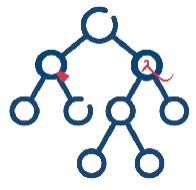
\includegraphics[height=1.0cm]{msca_logo.png}}%
    \end{center}

    \vspace{0.6cm}

    % Main title with Q logos on sides (with clickable links)
    \begin{center}
        \begin{minipage}{0.1\textwidth}
            \centering
            \href{https://quantlet.com}{
\includegraphics[height=1.1cm]{ql_logo.png}}
        \end{minipage}%
        \begin{minipage}{0.78\textwidth}
            \centering
            {\LARGE\bfseries\usebeamercolor[fg]{title}\inserttitle}

            \vspace{0.3cm}

            {\usebeamerfont{subtitle}\usebeamercolor[fg]{title}\insertsubtitle}
        \end{minipage}%
        \begin{minipage}{0.1\textwidth}
            \centering
            \href{https://quantinar.com}{
\includegraphics[height=1.1cm]{qr_logo.png}}
        \end{minipage}
    \end{center}

    \vspace{0.6cm}

    % Authors (left aligned)
    \hspace{0.5cm}{\usebeamerfont{author}\insertauthor}

    \vspace{0.3cm}

    % Institute/Affiliations (left aligned)
    \hspace{0.5cm}\begin{minipage}[t]{0.9\textwidth}
        \raggedright\small\insertinstitute
    \end{minipage}
}

%=============================================================================
% THEOREM ENVIRONMENTS
%=============================================================================
\theoremstyle{definition}
\setbeamertemplate{theorems}[numbered]
\ifdefined\atslang
\newtheorem{defn}{Definiție}
\newtheorem{thm}{Teoremă}
\newtheorem{prop}{Propoziție}
\newtheorem{rmk}{Observație}
\else
\newtheorem{defn}{Definition}
\newtheorem{thm}{Theorem}
\newtheorem{prop}{Proposition}
\newtheorem{rmk}{Remark}
\fi

%=============================================================================
% CENTRED MINIPAGE (no extra vertical space)
%=============================================================================
\newenvironment{cminipage}[1]{%
    \par\noindent\hfill\begin{minipage}{#1}\ignorespaces
}{%
    \end{minipage}\hfill\null\par
}

%=============================================================================
% CUSTOM COMMANDS
%=============================================================================
\newcommand{\E}{\mathbb{E}}
\newcommand{\Var}{\text{Var}}
\newcommand{\Cov}{\text{Cov}}
\newcommand{\Corr}{\text{Corr}}
\newcommand{\R}{\mathbb{R}}
\newcommand{\N}{\mathbb{N}}
\newcommand{\Z}{\mathbb{Z}}
\newcommand{\B}{\mathbf{B}}
\newcommand{\imark}{\textcolor{MainBlue}{\textbullet}}
\newcommand{\RMSE}{\text{RMSE}}
\newcommand{\MAE}{\text{MAE}}
\newcommand{\MAPE}{\text{MAPE}}

% Boldface vector/matrix commands (VAR, VECM, state space)
\newcommand{\bY}{\mathbf{Y}}
\newcommand{\bX}{\mathbf{X}}
\newcommand{\bA}{\mathbf{A}}
\newcommand{\bB}{\mathbf{B}}
\newcommand{\bepsilon}{\boldsymbol{\varepsilon}}
\newcommand{\bSigma}{\boldsymbol{\Sigma}}
\newcommand{\bPhi}{\boldsymbol{\Phi}}
\newcommand{\bGamma}{\boldsymbol{\Gamma}}
\newcommand{\bPi}{\boldsymbol{\Pi}}
\newcommand{\bc}{\mathbf{c}}
\newcommand{\balpha}{\boldsymbol{\alpha}}
\newcommand{\bbeta}{\boldsymbol{\beta}}
\newcommand{\bvarepsilon}{\boldsymbol{\varepsilon}}

% Seminar marks
\newcommand{\correct}{\textcolor{Forest}{\checkmark}}
\newcommand{\incorrect}{\textcolor{Crimson}{\texttimes}}
 se definește
%   \newcommand{\coursename}{Advanced Time Series Analysis and Forecasting}          (EN)
%   \newcommand{\coursename}{Analiza avansată a seriilor de timp și previziune}       (RO)  și  \def\atslang{ro}
% Fișierele .tex se află în EN/Courses, EN/Seminars, RO/Cursuri, RO/Seminarii (două niveluri sub rădăcină).
% Deck-urile sînt generate de latex/build_chapterN.py / build_seminarN.py (vezi latex/ats_build.py).

\documentclass[9pt, aspectratio=169, t]{beamer}
\providecommand{\coursename}{Advanced Time Series Analysis and Forecasting}

% Ensure content fits on slides
\setbeamersize{text margin left=8mm, text margin right=8mm}
% Smaller institute font (title page)
\setbeamerfont{institute}{size=\footnotesize}

%=============================================================================
% THEME AND STYLE CONFIGURATION
%=============================================================================
\usetheme{default}
% Using default theme for clean header/footer control

% Color Palette (matching Redispatch PDF)
\definecolor{MainBlue}{RGB}{26, 58, 110}
\definecolor{AccentBlue}{RGB}{26, 58, 110}
\definecolor{IDAred}{RGB}{205, 0, 0}
\definecolor{DarkGray}{RGB}{51, 51, 51}
\definecolor{MediumGray}{RGB}{128, 128, 128}
\definecolor{LightGray}{RGB}{248, 248, 248}
\definecolor{VeryLightGray}{RGB}{235, 235, 235}
\definecolor{KeynoteGray}{RGB}{218, 218, 218}
\definecolor{SectionGray}{RGB}{120, 120, 120}
\definecolor{FooterGray}{RGB}{100, 100, 100}
\definecolor{Crimson}{RGB}{220, 53, 69}
\definecolor{Forest}{RGB}{46, 125, 50}
\definecolor{Amber}{RGB}{181, 133, 63}
\definecolor{Orange}{RGB}{230, 126, 34}
\definecolor{Purple}{RGB}{142, 68, 173}

% Gradient background (exact Keynote 315° gradient: white to RGB 218,218,218)
\setbeamertemplate{background}{%
    \begin{tikzpicture}[remember picture, overlay]
        \shade[shading=axis, shading angle=315,
        top color=white, bottom color=KeynoteGray]
        (current page.south west) rectangle (current page.north east);
    \end{tikzpicture}%
}
% Fallback solid color for compatibility
\setbeamercolor{background canvas}{bg=}

\setbeamercolor{palette primary}{bg=MainBlue, fg=white}
\setbeamercolor{palette secondary}{bg=MainBlue!85, fg=white}
\setbeamercolor{palette tertiary}{bg=MainBlue!70, fg=white}
\setbeamercolor{structure}{fg=MainBlue}
\setbeamercolor{title}{fg=IDAred}
\setbeamercolor{frametitle}{fg=IDAred, bg=}
\setbeamercolor{block title}{bg=MainBlue, fg=white}
\setbeamercolor{block body}{bg=VeryLightGray, fg=DarkGray}
\setbeamercolor{block title alerted}{bg=Crimson, fg=white}
\setbeamercolor{block body alerted}{bg=Crimson!8, fg=DarkGray}
\setbeamercolor{block title example}{bg=Forest, fg=white}
\setbeamercolor{block body example}{bg=Forest!8, fg=DarkGray}
\setbeamercolor{item}{fg=MainBlue}

% Footer colors (override Madrid theme blue)
\setbeamercolor{author in head/foot}{fg=FooterGray, bg=}
\setbeamercolor{title in head/foot}{fg=FooterGray, bg=}
\setbeamercolor{date in head/foot}{fg=FooterGray, bg=}
\setbeamercolor{section in head/foot}{fg=FooterGray, bg=}
\setbeamercolor{subsection in head/foot}{fg=FooterGray, bg=}

% Bullet styles (apply everywhere including blocks)
\setbeamertemplate{itemize item}{\color{MainBlue}$\boxdot$}
\setbeamertemplate{itemize subitem}{\color{MainBlue}$\blacktriangleright$}
\setbeamertemplate{itemize subsubitem}{\color{MainBlue}\tiny$\bullet$}
\setbeamertemplate{itemize/enumerate body begin}{\normalsize}
\setbeamertemplate{itemize/enumerate subbody begin}{\normalsize}

% Item spacing - compact style
\setlength{\leftmargini}{10pt}       % Level 1: minimal indent
\setlength{\leftmarginii}{10pt}      % Level 2: minimal additional indent
% Compact list spacing (zero extra space before/after lists in blocks)
\makeatletter
\def\@listi{\leftmargin\leftmargini \topsep 0pt \parsep 0pt \itemsep 0pt}
\def\@listii{\leftmargin\leftmarginii \topsep 0pt \parsep 0pt \itemsep 0pt}
\makeatother

\setbeamertemplate{navigation symbols}{}

%=============================================================================
% CUSTOM HEADLINE
%=============================================================================
\setbeamertemplate{headline}{%
    \vskip10pt%
    \hbox to \paperwidth{%
        \hskip0.5cm%
        {\small\color{FooterGray}\renewcommand{\hyperlink}[2]{##2}\insertsectionhead}%
        \hfill%
        \textcolor{FooterGray}{\small\insertframenumber}%
        \hskip0.5cm%
    }%
    \vskip4pt%
    {\color{FooterGray}\hrule height 0.4pt}%
}

%=============================================================================
% CUSTOM FOOTER
%=============================================================================
\usepackage{fontawesome5}

\setbeamertemplate{footline}{%
    {\color{FooterGray}\hrule height 0.4pt}%
    \vskip4pt%
    \hbox to \paperwidth{%
        \hskip0.5cm%
        \textcolor{FooterGray}{\small\coursename}%
        \hfill%
        \raisebox{-0.1em}{%
            \begin{tikzpicture}[x=0.08em, y=0.08em, line width=0.4pt]
                \draw[FooterGray] (0,3) -- (1,4) -- (2,3.5) -- (3,5) -- (4,4) -- (5,6) -- (6,5.5) -- (7,4) -- (8,5) -- (9,7) -- (10,6) -- (11,5) -- (12,6.5) -- (13,8) -- (14,7) -- (15,6) -- (16,7.5) -- (17,9) -- (18,8) -- (19,7) -- (20,8.5) -- (21,10) -- (22,9) -- (23,8) -- (24,9.5);
            \end{tikzpicture}%
        }%
        \hskip0.5cm%
    }%
    \vskip6pt%
}

%=============================================================================
% PACKAGES
%=============================================================================
\usepackage[utf8]{inputenc}
\DeclareUnicodeCharacter{03B1}{\ensuremath{\alpha}}
\usepackage[T1]{fontenc}
\usepackage{amsmath, amssymb, amsthm}
\usepackage{mathtools}
\usepackage{bm}
\usepackage{tikz}
\usetikzlibrary{arrows.meta, positioning, shapes, calc, decorations.pathreplacing, shadings}
\usepackage{booktabs}
\usepackage{multirow}
\usepackage{array}
\usepackage{graphicx}
\usepackage{animate}
\usepackage{hyperref}
\usepackage{colortbl}
\usepackage{listings}
\lstset{language=Python, basicstyle=\ttfamily\scriptsize, keywordstyle=\color{MainBlue}\bfseries,
  commentstyle=\color{Forest}, stringstyle=\color{Crimson}, breaklines=true,
  frame=none, backgroundcolor=\color{VeryLightGray}, xleftmargin=2mm}
\hypersetup{colorlinks=true, linkcolor=MainBlue, urlcolor=MainBlue}
\graphicspath{{../../logos/}{../../charts/}{../../photos/}}
\usepackage{xcolor}
\hfuzz=2pt  % Suppress tiny overfull warnings (<2pt)
\vfuzz=2pt  % Suppress tiny vertical overfull warnings (<2pt)

%=============================================================================
% QUANTLET COMMANDS
%   \quantlet{<displayed name>}{<url>}       (generic)
%   \atsquantlet{Ch_05}{ATS_ch5_garch}       -> https://github.com/danpele/Advanced-Time-Series/tree/main/Quantlets/Ch_05/ATS_ch5_garch
%   \qlurl{<folder>} is defined per chapter by the generator (Quantlets/Ch_NN/<folder>)
%=============================================================================
\newcommand{\atsrepo}{https://github.com/danpele/Advanced-Time-Series}
\newcommand{\atsqlbase}{https://github.com/danpele/Advanced-Time-Series/tree/main/Quantlets}
\newcommand{\quantlet}[2]{%
    \hfill\href{#2}{%
        \raisebox{-0.15em}{
\includegraphics[height=0.7em]{ql_logo.png}}%
        \textcolor{MainBlue}{\tiny\ #1}%
    }%
}
\newcommand{\atsquantlet}[2]{\quantlet{\detokenize{#2}}{\atsqlbase/#1/#2}}

%=============================================================================
% NOTEBOOKS (Google Colab)
%   \colaburl{notebooks/EN/chapter5_seminar_notebook.ipynb} -> the Colab link of a file in the ATS repo
%   \nb: the chapter notebook (each seminar deck redefines it with \renewcommand)
%=============================================================================
\newcommand{\colaburl}[1]{https://colab.research.google.com/github/danpele/Advanced-Time-Series/blob/main/#1}
\newcommand{\nb}{https://colab.research.google.com/github/danpele/Advanced-Time-Series/tree/main/notebooks/EN}
\newcommand{\nbname}{notebooks/EN}

%=============================================================================
% SLIDE HELPERS (used by the generators; the same as in MFM)
%=============================================================================
% local font size for list bodies (the preamble forces \normalsize)
\newcommand{\itemsize}[1]{\setbeamertemplate{itemize/enumerate body begin}{#1}\setbeamertemplate{itemize/enumerate subbody begin}{#1}}
\newcommand{\intitle}[1]{{\hypersetup{urlcolor=white}#1}}   % white links inside coloured title bars
\newcommand{\imgcap}[1]{{\scriptsize #1}\\[0.5mm]}          % caption under a photo
\newcommand{\imgcredit}[2]{{\tiny\color{FooterGray}\href{#1}{#2}}}   % image credit: source URL, author/licence
\newcommand{\aiprompt}[1]{{\ttfamily\color{MainBlue}#1}}     % a prompt to an AI assistant

%=============================================================================
% SEMINARS: student version by default; the instructor wrapper *_solutions.tex sets \solutionstrue
%=============================================================================
\makeatletter\@ifundefined{ifsolutions}{\expandafter\newif\csname ifsolutions\endcsname}{}\makeatother
\newcommand{\solonly}[1]{\ifsolutions #1\fi}
\newcommand{\propsub}{\ifsolutions\else\framesubtitle{\ifdefined\atslang Rezolvarea se discută la seminar\else Solution discussed in class\fi}\fi}

%=============================================================================
% APPENDIX AND CHAPTER LINKS (latex/appendix_links.py writes the calls; it also re-declares these
% macros before \begin{document}, so the decks compile with or without this preamble block)
%=============================================================================
\providecommand{\atsapplink}[3]{\hypertarget{#2}{}\hyperlink{#1}{\beamergotobutton{#3}}}
\providecommand{\atsappback}[2]{\begin{tikzpicture}[remember picture,overlay]\node[anchor=south east] at ([xshift=-3mm,yshift=7mm]current page.south east){\hyperlink{#1}{\beamerreturnbutton{#2}}};\end{tikzpicture}}
\providecommand{\atschlink}[2]{\href{#1}{#2}}
\providecommand{\atschlinkt}[2]{\href{#1}{\usebeamercolor[fg]{frametitle}#2}}

%=============================================================================
% QUANTINAR COMMAND: link către un curs Quantinar (subiecte avansate)
%=============================================================================
\newcommand{\quantinar}[2]{%
    \href{#2}{%
        \raisebox{-0.15em}{
\includegraphics[height=0.8em]{qr_logo.png}}%
        \textcolor{MainBlue}{\scriptsize\ #1}%
    }%
}

%=============================================================================
% CUSTOM TITLE PAGE
%=============================================================================
\defbeamertemplate*{title page}{hybrid}[1][]
{
    \vspace{0.2cm}
    % Logos row - top header (with clickable links)
    \begin{center}
        \href{https://www.ase.ro}{
\includegraphics[height=1.0cm]{ase_logo.png}}\hspace{0.3cm}%
        \href{https://theida.net}{
\includegraphics[height=1.0cm]{ida_logo.png}}\hspace{0.3cm}%
        \href{https://blockchain-research-center.com}{
\includegraphics[height=1.0cm]{brc_logo.png}}\hspace{0.3cm}%
        \href{https://www.ai4efin.ase.ro}{
\includegraphics[height=1.0cm]{ai4efin_logo.png}}\hspace{0.3cm}%
        \href{https://ipe.ro/new}{
\includegraphics[height=1.0cm]{acad_logo.png}}\hspace{0.3cm}%
        \href{https://www.digital-finance-msca.com}{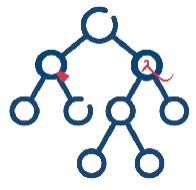
\includegraphics[height=1.0cm]{msca_logo.png}}%
    \end{center}

    \vspace{0.6cm}

    % Main title with Q logos on sides (with clickable links)
    \begin{center}
        \begin{minipage}{0.1\textwidth}
            \centering
            \href{https://quantlet.com}{
\includegraphics[height=1.1cm]{ql_logo.png}}
        \end{minipage}%
        \begin{minipage}{0.78\textwidth}
            \centering
            {\LARGE\bfseries\usebeamercolor[fg]{title}\inserttitle}

            \vspace{0.3cm}

            {\usebeamerfont{subtitle}\usebeamercolor[fg]{title}\insertsubtitle}
        \end{minipage}%
        \begin{minipage}{0.1\textwidth}
            \centering
            \href{https://quantinar.com}{
\includegraphics[height=1.1cm]{qr_logo.png}}
        \end{minipage}
    \end{center}

    \vspace{0.6cm}

    % Authors (left aligned)
    \hspace{0.5cm}{\usebeamerfont{author}\insertauthor}

    \vspace{0.3cm}

    % Institute/Affiliations (left aligned)
    \hspace{0.5cm}\begin{minipage}[t]{0.9\textwidth}
        \raggedright\small\insertinstitute
    \end{minipage}
}

%=============================================================================
% THEOREM ENVIRONMENTS
%=============================================================================
\theoremstyle{definition}
\setbeamertemplate{theorems}[numbered]
\ifdefined\atslang
\newtheorem{defn}{Definiție}
\newtheorem{thm}{Teoremă}
\newtheorem{prop}{Propoziție}
\newtheorem{rmk}{Observație}
\else
\newtheorem{defn}{Definition}
\newtheorem{thm}{Theorem}
\newtheorem{prop}{Proposition}
\newtheorem{rmk}{Remark}
\fi

%=============================================================================
% CENTRED MINIPAGE (no extra vertical space)
%=============================================================================
\newenvironment{cminipage}[1]{%
    \par\noindent\hfill\begin{minipage}{#1}\ignorespaces
}{%
    \end{minipage}\hfill\null\par
}

%=============================================================================
% CUSTOM COMMANDS
%=============================================================================
\newcommand{\E}{\mathbb{E}}
\newcommand{\Var}{\text{Var}}
\newcommand{\Cov}{\text{Cov}}
\newcommand{\Corr}{\text{Corr}}
\newcommand{\R}{\mathbb{R}}
\newcommand{\N}{\mathbb{N}}
\newcommand{\Z}{\mathbb{Z}}
\newcommand{\B}{\mathbf{B}}
\newcommand{\imark}{\textcolor{MainBlue}{\textbullet}}
\newcommand{\RMSE}{\text{RMSE}}
\newcommand{\MAE}{\text{MAE}}
\newcommand{\MAPE}{\text{MAPE}}

% Boldface vector/matrix commands (VAR, VECM, state space)
\newcommand{\bY}{\mathbf{Y}}
\newcommand{\bX}{\mathbf{X}}
\newcommand{\bA}{\mathbf{A}}
\newcommand{\bB}{\mathbf{B}}
\newcommand{\bepsilon}{\boldsymbol{\varepsilon}}
\newcommand{\bSigma}{\boldsymbol{\Sigma}}
\newcommand{\bPhi}{\boldsymbol{\Phi}}
\newcommand{\bGamma}{\boldsymbol{\Gamma}}
\newcommand{\bPi}{\boldsymbol{\Pi}}
\newcommand{\bc}{\mathbf{c}}
\newcommand{\balpha}{\boldsymbol{\alpha}}
\newcommand{\bbeta}{\boldsymbol{\beta}}
\newcommand{\bvarepsilon}{\boldsymbol{\varepsilon}}

% Seminar marks
\newcommand{\correct}{\textcolor{Forest}{\checkmark}}
\newcommand{\incorrect}{\textcolor{Crimson}{\texttimes}}
 se definește
%   \newcommand{\coursename}{Advanced Time Series Analysis and Forecasting}          (EN)
%   \newcommand{\coursename}{Analiza avansată a seriilor de timp și previziune}       (RO)  și  \def\atslang{ro}
% Fișierele .tex se află în EN/Courses, EN/Seminars, RO/Cursuri, RO/Seminarii (două niveluri sub rădăcină).
% Deck-urile sînt generate de latex/build_chapterN.py / build_seminarN.py (vezi latex/ats_build.py).

\documentclass[9pt, aspectratio=169, t]{beamer}
\providecommand{\coursename}{Advanced Time Series Analysis and Forecasting}

% Ensure content fits on slides
\setbeamersize{text margin left=8mm, text margin right=8mm}
% Smaller institute font (title page)
\setbeamerfont{institute}{size=\footnotesize}

%=============================================================================
% THEME AND STYLE CONFIGURATION
%=============================================================================
\usetheme{default}
% Using default theme for clean header/footer control

% Color Palette (matching Redispatch PDF)
\definecolor{MainBlue}{RGB}{26, 58, 110}
\definecolor{AccentBlue}{RGB}{26, 58, 110}
\definecolor{IDAred}{RGB}{205, 0, 0}
\definecolor{DarkGray}{RGB}{51, 51, 51}
\definecolor{MediumGray}{RGB}{128, 128, 128}
\definecolor{LightGray}{RGB}{248, 248, 248}
\definecolor{VeryLightGray}{RGB}{235, 235, 235}
\definecolor{KeynoteGray}{RGB}{218, 218, 218}
\definecolor{SectionGray}{RGB}{120, 120, 120}
\definecolor{FooterGray}{RGB}{100, 100, 100}
\definecolor{Crimson}{RGB}{220, 53, 69}
\definecolor{Forest}{RGB}{46, 125, 50}
\definecolor{Amber}{RGB}{181, 133, 63}
\definecolor{Orange}{RGB}{230, 126, 34}
\definecolor{Purple}{RGB}{142, 68, 173}

% Gradient background (exact Keynote 315° gradient: white to RGB 218,218,218)
\setbeamertemplate{background}{%
    \begin{tikzpicture}[remember picture, overlay]
        \shade[shading=axis, shading angle=315,
        top color=white, bottom color=KeynoteGray]
        (current page.south west) rectangle (current page.north east);
    \end{tikzpicture}%
}
% Fallback solid color for compatibility
\setbeamercolor{background canvas}{bg=}

\setbeamercolor{palette primary}{bg=MainBlue, fg=white}
\setbeamercolor{palette secondary}{bg=MainBlue!85, fg=white}
\setbeamercolor{palette tertiary}{bg=MainBlue!70, fg=white}
\setbeamercolor{structure}{fg=MainBlue}
\setbeamercolor{title}{fg=IDAred}
\setbeamercolor{frametitle}{fg=IDAred, bg=}
\setbeamercolor{block title}{bg=MainBlue, fg=white}
\setbeamercolor{block body}{bg=VeryLightGray, fg=DarkGray}
\setbeamercolor{block title alerted}{bg=Crimson, fg=white}
\setbeamercolor{block body alerted}{bg=Crimson!8, fg=DarkGray}
\setbeamercolor{block title example}{bg=Forest, fg=white}
\setbeamercolor{block body example}{bg=Forest!8, fg=DarkGray}
\setbeamercolor{item}{fg=MainBlue}

% Footer colors (override Madrid theme blue)
\setbeamercolor{author in head/foot}{fg=FooterGray, bg=}
\setbeamercolor{title in head/foot}{fg=FooterGray, bg=}
\setbeamercolor{date in head/foot}{fg=FooterGray, bg=}
\setbeamercolor{section in head/foot}{fg=FooterGray, bg=}
\setbeamercolor{subsection in head/foot}{fg=FooterGray, bg=}

% Bullet styles (apply everywhere including blocks)
\setbeamertemplate{itemize item}{\color{MainBlue}$\boxdot$}
\setbeamertemplate{itemize subitem}{\color{MainBlue}$\blacktriangleright$}
\setbeamertemplate{itemize subsubitem}{\color{MainBlue}\tiny$\bullet$}
\setbeamertemplate{itemize/enumerate body begin}{\normalsize}
\setbeamertemplate{itemize/enumerate subbody begin}{\normalsize}

% Item spacing - compact style
\setlength{\leftmargini}{10pt}       % Level 1: minimal indent
\setlength{\leftmarginii}{10pt}      % Level 2: minimal additional indent
% Compact list spacing (zero extra space before/after lists in blocks)
\makeatletter
\def\@listi{\leftmargin\leftmargini \topsep 0pt \parsep 0pt \itemsep 0pt}
\def\@listii{\leftmargin\leftmarginii \topsep 0pt \parsep 0pt \itemsep 0pt}
\makeatother

\setbeamertemplate{navigation symbols}{}

%=============================================================================
% CUSTOM HEADLINE
%=============================================================================
\setbeamertemplate{headline}{%
    \vskip10pt%
    \hbox to \paperwidth{%
        \hskip0.5cm%
        {\small\color{FooterGray}\renewcommand{\hyperlink}[2]{##2}\insertsectionhead}%
        \hfill%
        \textcolor{FooterGray}{\small\insertframenumber}%
        \hskip0.5cm%
    }%
    \vskip4pt%
    {\color{FooterGray}\hrule height 0.4pt}%
}

%=============================================================================
% CUSTOM FOOTER
%=============================================================================
\usepackage{fontawesome5}

\setbeamertemplate{footline}{%
    {\color{FooterGray}\hrule height 0.4pt}%
    \vskip4pt%
    \hbox to \paperwidth{%
        \hskip0.5cm%
        \textcolor{FooterGray}{\small\coursename}%
        \hfill%
        \raisebox{-0.1em}{%
            \begin{tikzpicture}[x=0.08em, y=0.08em, line width=0.4pt]
                \draw[FooterGray] (0,3) -- (1,4) -- (2,3.5) -- (3,5) -- (4,4) -- (5,6) -- (6,5.5) -- (7,4) -- (8,5) -- (9,7) -- (10,6) -- (11,5) -- (12,6.5) -- (13,8) -- (14,7) -- (15,6) -- (16,7.5) -- (17,9) -- (18,8) -- (19,7) -- (20,8.5) -- (21,10) -- (22,9) -- (23,8) -- (24,9.5);
            \end{tikzpicture}%
        }%
        \hskip0.5cm%
    }%
    \vskip6pt%
}

%=============================================================================
% PACKAGES
%=============================================================================
\usepackage[utf8]{inputenc}
\DeclareUnicodeCharacter{03B1}{\ensuremath{\alpha}}
\usepackage[T1]{fontenc}
\usepackage{amsmath, amssymb, amsthm}
\usepackage{mathtools}
\usepackage{bm}
\usepackage{tikz}
\usetikzlibrary{arrows.meta, positioning, shapes, calc, decorations.pathreplacing, shadings}
\usepackage{booktabs}
\usepackage{multirow}
\usepackage{array}
\usepackage{graphicx}
\usepackage{animate}
\usepackage{hyperref}
\usepackage{colortbl}
\usepackage{listings}
\lstset{language=Python, basicstyle=\ttfamily\scriptsize, keywordstyle=\color{MainBlue}\bfseries,
  commentstyle=\color{Forest}, stringstyle=\color{Crimson}, breaklines=true,
  frame=none, backgroundcolor=\color{VeryLightGray}, xleftmargin=2mm}
\hypersetup{colorlinks=true, linkcolor=MainBlue, urlcolor=MainBlue}
\graphicspath{{../../logos/}{../../charts/}{../../photos/}}
\usepackage{xcolor}
\hfuzz=2pt  % Suppress tiny overfull warnings (<2pt)
\vfuzz=2pt  % Suppress tiny vertical overfull warnings (<2pt)

%=============================================================================
% QUANTLET COMMANDS
%   \quantlet{<displayed name>}{<url>}       (generic)
%   \atsquantlet{Ch_05}{ATS_ch5_garch}       -> https://github.com/danpele/Advanced-Time-Series/tree/main/Quantlets/Ch_05/ATS_ch5_garch
%   \qlurl{<folder>} is defined per chapter by the generator (Quantlets/Ch_NN/<folder>)
%=============================================================================
\newcommand{\atsrepo}{https://github.com/danpele/Advanced-Time-Series}
\newcommand{\atsqlbase}{https://github.com/danpele/Advanced-Time-Series/tree/main/Quantlets}
\newcommand{\quantlet}[2]{%
    \hfill\href{#2}{%
        \raisebox{-0.15em}{
\includegraphics[height=0.7em]{ql_logo.png}}%
        \textcolor{MainBlue}{\tiny\ #1}%
    }%
}
\newcommand{\atsquantlet}[2]{\quantlet{\detokenize{#2}}{\atsqlbase/#1/#2}}

%=============================================================================
% NOTEBOOKS (Google Colab)
%   \colaburl{notebooks/EN/chapter5_seminar_notebook.ipynb} -> the Colab link of a file in the ATS repo
%   \nb: the chapter notebook (each seminar deck redefines it with \renewcommand)
%=============================================================================
\newcommand{\colaburl}[1]{https://colab.research.google.com/github/danpele/Advanced-Time-Series/blob/main/#1}
\newcommand{\nb}{https://colab.research.google.com/github/danpele/Advanced-Time-Series/tree/main/notebooks/EN}
\newcommand{\nbname}{notebooks/EN}

%=============================================================================
% SLIDE HELPERS (used by the generators; the same as in MFM)
%=============================================================================
% local font size for list bodies (the preamble forces \normalsize)
\newcommand{\itemsize}[1]{\setbeamertemplate{itemize/enumerate body begin}{#1}\setbeamertemplate{itemize/enumerate subbody begin}{#1}}
\newcommand{\intitle}[1]{{\hypersetup{urlcolor=white}#1}}   % white links inside coloured title bars
\newcommand{\imgcap}[1]{{\scriptsize #1}\\[0.5mm]}          % caption under a photo
\newcommand{\imgcredit}[2]{{\tiny\color{FooterGray}\href{#1}{#2}}}   % image credit: source URL, author/licence
\newcommand{\aiprompt}[1]{{\ttfamily\color{MainBlue}#1}}     % a prompt to an AI assistant

%=============================================================================
% SEMINARS: student version by default; the instructor wrapper *_solutions.tex sets \solutionstrue
%=============================================================================
\makeatletter\@ifundefined{ifsolutions}{\expandafter\newif\csname ifsolutions\endcsname}{}\makeatother
\newcommand{\solonly}[1]{\ifsolutions #1\fi}
\newcommand{\propsub}{\ifsolutions\else\framesubtitle{\ifdefined\atslang Rezolvarea se discută la seminar\else Solution discussed in class\fi}\fi}

%=============================================================================
% APPENDIX AND CHAPTER LINKS (latex/appendix_links.py writes the calls; it also re-declares these
% macros before \begin{document}, so the decks compile with or without this preamble block)
%=============================================================================
\providecommand{\atsapplink}[3]{\hypertarget{#2}{}\hyperlink{#1}{\beamergotobutton{#3}}}
\providecommand{\atsappback}[2]{\begin{tikzpicture}[remember picture,overlay]\node[anchor=south east] at ([xshift=-3mm,yshift=7mm]current page.south east){\hyperlink{#1}{\beamerreturnbutton{#2}}};\end{tikzpicture}}
\providecommand{\atschlink}[2]{\href{#1}{#2}}
\providecommand{\atschlinkt}[2]{\href{#1}{\usebeamercolor[fg]{frametitle}#2}}

%=============================================================================
% QUANTINAR COMMAND: link către un curs Quantinar (subiecte avansate)
%=============================================================================
\newcommand{\quantinar}[2]{%
    \href{#2}{%
        \raisebox{-0.15em}{
\includegraphics[height=0.8em]{qr_logo.png}}%
        \textcolor{MainBlue}{\scriptsize\ #1}%
    }%
}

%=============================================================================
% CUSTOM TITLE PAGE
%=============================================================================
\defbeamertemplate*{title page}{hybrid}[1][]
{
    \vspace{0.2cm}
    % Logos row - top header (with clickable links)
    \begin{center}
        \href{https://www.ase.ro}{
\includegraphics[height=1.0cm]{ase_logo.png}}\hspace{0.3cm}%
        \href{https://theida.net}{
\includegraphics[height=1.0cm]{ida_logo.png}}\hspace{0.3cm}%
        \href{https://blockchain-research-center.com}{
\includegraphics[height=1.0cm]{brc_logo.png}}\hspace{0.3cm}%
        \href{https://www.ai4efin.ase.ro}{
\includegraphics[height=1.0cm]{ai4efin_logo.png}}\hspace{0.3cm}%
        \href{https://ipe.ro/new}{
\includegraphics[height=1.0cm]{acad_logo.png}}\hspace{0.3cm}%
        \href{https://www.digital-finance-msca.com}{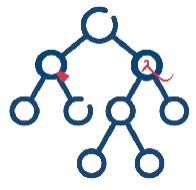
\includegraphics[height=1.0cm]{msca_logo.png}}%
    \end{center}

    \vspace{0.6cm}

    % Main title with Q logos on sides (with clickable links)
    \begin{center}
        \begin{minipage}{0.1\textwidth}
            \centering
            \href{https://quantlet.com}{
\includegraphics[height=1.1cm]{ql_logo.png}}
        \end{minipage}%
        \begin{minipage}{0.78\textwidth}
            \centering
            {\LARGE\bfseries\usebeamercolor[fg]{title}\inserttitle}

            \vspace{0.3cm}

            {\usebeamerfont{subtitle}\usebeamercolor[fg]{title}\insertsubtitle}
        \end{minipage}%
        \begin{minipage}{0.1\textwidth}
            \centering
            \href{https://quantinar.com}{
\includegraphics[height=1.1cm]{qr_logo.png}}
        \end{minipage}
    \end{center}

    \vspace{0.6cm}

    % Authors (left aligned)
    \hspace{0.5cm}{\usebeamerfont{author}\insertauthor}

    \vspace{0.3cm}

    % Institute/Affiliations (left aligned)
    \hspace{0.5cm}\begin{minipage}[t]{0.9\textwidth}
        \raggedright\small\insertinstitute
    \end{minipage}
}

%=============================================================================
% THEOREM ENVIRONMENTS
%=============================================================================
\theoremstyle{definition}
\setbeamertemplate{theorems}[numbered]
\ifdefined\atslang
\newtheorem{defn}{Definiție}
\newtheorem{thm}{Teoremă}
\newtheorem{prop}{Propoziție}
\newtheorem{rmk}{Observație}
\else
\newtheorem{defn}{Definition}
\newtheorem{thm}{Theorem}
\newtheorem{prop}{Proposition}
\newtheorem{rmk}{Remark}
\fi

%=============================================================================
% CENTRED MINIPAGE (no extra vertical space)
%=============================================================================
\newenvironment{cminipage}[1]{%
    \par\noindent\hfill\begin{minipage}{#1}\ignorespaces
}{%
    \end{minipage}\hfill\null\par
}

%=============================================================================
% CUSTOM COMMANDS
%=============================================================================
\newcommand{\E}{\mathbb{E}}
\newcommand{\Var}{\text{Var}}
\newcommand{\Cov}{\text{Cov}}
\newcommand{\Corr}{\text{Corr}}
\newcommand{\R}{\mathbb{R}}
\newcommand{\N}{\mathbb{N}}
\newcommand{\Z}{\mathbb{Z}}
\newcommand{\B}{\mathbf{B}}
\newcommand{\imark}{\textcolor{MainBlue}{\textbullet}}
\newcommand{\RMSE}{\text{RMSE}}
\newcommand{\MAE}{\text{MAE}}
\newcommand{\MAPE}{\text{MAPE}}

% Boldface vector/matrix commands (VAR, VECM, state space)
\newcommand{\bY}{\mathbf{Y}}
\newcommand{\bX}{\mathbf{X}}
\newcommand{\bA}{\mathbf{A}}
\newcommand{\bB}{\mathbf{B}}
\newcommand{\bepsilon}{\boldsymbol{\varepsilon}}
\newcommand{\bSigma}{\boldsymbol{\Sigma}}
\newcommand{\bPhi}{\boldsymbol{\Phi}}
\newcommand{\bGamma}{\boldsymbol{\Gamma}}
\newcommand{\bPi}{\boldsymbol{\Pi}}
\newcommand{\bc}{\mathbf{c}}
\newcommand{\balpha}{\boldsymbol{\alpha}}
\newcommand{\bbeta}{\boldsymbol{\beta}}
\newcommand{\bvarepsilon}{\boldsymbol{\varepsilon}}

% Seminar marks
\newcommand{\correct}{\textcolor{Forest}{\checkmark}}
\newcommand{\incorrect}{\textcolor{Crimson}{\texttimes}}


\newcommand{\qlurl}[1]{https://github.com/danpele/Advanced-Time-Series/tree/main/Quantlets/Ch_04/#1}

% Clickable citations (DOIs verified via Crossref)
\newcommand{\refAL}{\href{https://doi.org/10.1177/1536867X1601600314}{Abrigo and Love (2016)}}
\newcommand{\refBac}{\href{https://doi.org/10.1016/0140-9883(91)90022-R}{Bacon (1991)}}
\newcommand{\refBrP}{\href{https://doi.org/10.1007/978-3-540-75892-1_9}{Breitung and Pesaran (2008)}}
\newcommand{\refCRTa}{\href{https://doi.org/10.1017/S0266466609990776}{Cavaliere, Rahbek and Taylor (2010)}}
\newcommand{\refCRT}{\href{https://doi.org/10.3982/ECTA9099}{Cavaliere, Rahbek and Taylor (2012)}}
\newcommand{\refCP}{\href{https://doi.org/10.1016/j.jeconom.2015.03.007}{Chudik and Pesaran (2015)}}
\newcommand{\refdB}{\href{https://doi.org/10.1111/j.1465-6485.2005.00121.x}{de Bondt (2005)}}
\newcommand{\refECR}{\href{https://doi.org/10.1016/j.jpolmod.2007.01.005}{Égert, Crespo-Cuaresma and Reininger (2007)}}
\newcommand{\refEG}{\href{https://doi.org/10.2307/1913236}{Engle and Granger (1987)}}
\newcommand{\refGN}{\href{https://doi.org/10.1016/S0165-1889(99)00062-7}{Gonzalo and Ng (2001)}}
\newcommand{\refHam}{\href{https://doi.org/10.2307/j.ctv14jx6sm}{Hamilton (1994)}}
\newcommand{\refHNR}{\href{https://doi.org/10.2307/1913103}{Holtz-Eakin, Newey and Rosen (1988)}}
\newcommand{\refIPS}{\href{https://doi.org/10.1016/S0304-4076(03)00092-7}{Im, Pesaran and Shin (2003)}}
\newcommand{\refJohA}{\href{https://doi.org/10.1016/0165-1889(88)90041-3}{Johansen (1988)}}
\newcommand{\refJohB}{\href{https://doi.org/10.2307/2938278}{Johansen (1991)}}
\newcommand{\refJohC}{\href{https://doi.org/10.1111/j.1468-0084.1992.tb00008.x}{Johansen (1992)}}
\newcommand{\refJohD}{\href{https://doi.org/10.1093/0198774508.001.0001}{Johansen (1995a)}}
\newcommand{\refJohE}{\href{https://doi.org/10.1016/0304-4076(94)01664-L}{Johansen (1995b)}}
\newcommand{\refJohF}{\href{https://doi.org/10.1017/S0266466600009026}{Johansen (1995c)}}
\newcommand{\refJohG}{\href{https://doi.org/10.1111/1468-0262.00358}{Johansen (2002)}}
\newcommand{\refJJ}{\href{https://doi.org/10.1111/j.1468-0084.1990.mp52002003.x}{Johansen and Juselius (1990)}}
\newcommand{\refJMN}{\href{https://doi.org/10.1111/1368-423X.00047}{Johansen, Mosconi and Nielsen (2000)}}
\newcommand{\refJus}{\href{https://doi.org/10.1093/oso/9780199285662.001.0001}{Juselius (2006)}}
\newcommand{\refKao}{\href{https://doi.org/10.1016/S0304-4076(98)00023-2}{Kao (1999)}}
\newcommand{\refKPY}{\href{https://doi.org/10.1016/j.jeconom.2010.10.001}{Kapetanios, Pesaran and Yamagata (2011)}}
\newcommand{\refKL}{\href{https://doi.org/10.1017/9781108164818}{Kilian and Lütkepohl (2017)}}
\newcommand{\refKPSW}{\href{https://www.jstor.org/stable/2006644}{King, Plosser, Stock and Watson (1991)}}
\newcommand{\refKS}{\href{https://doi.org/10.1111/obes.12377}{Kripfganz and Schneider (2020)}}
\newcommand{\refLLC}{\href{https://doi.org/10.1016/S0304-4076(01)00098-7}{Levin, Lin and Chu (2002)}}
\newcommand{\refLut}{\href{https://doi.org/10.1007/978-3-540-27752-1}{Lütkepohl (2005)}}
\newcommand{\refMHM}{\href{https://doi.org/10.1002/(SICI)1099-1255(199909/10)14:5\%3C563::AID-JAE530\%3E3.0.CO\%3B2-R}{MacKinnon, Haug and Michelis (1999)}}
\newcommand{\refNar}{\href{https://doi.org/10.1080/00036840500278103}{Narayan (2005)}}
\newcommand{\refNic}{\href{https://doi.org/10.2307/1911408}{Nickell (1981)}}
\newcommand{\refOL}{\href{https://doi.org/10.1111/j.1468-0084.1992.tb00013.x}{Osterwald-Lenum (1992)}}
\newcommand{\refPan}{\href{https://doi.org/10.1017/S0266466600012421}{Pantula (1989)}}
\newcommand{\refPedA}{\href{https://doi.org/10.1111/1468-0084.0610s1653}{Pedroni (1999)}}
\newcommand{\refPedB}{\href{https://doi.org/10.1162/003465301753237803}{Pedroni (2001)}}
\newcommand{\refPedC}{\href{https://doi.org/10.1017/S0266466604203073}{Pedroni (2004)}}
\newcommand{\refPesA}{\href{https://doi.org/10.1111/j.1468-0262.2006.00692.x}{Pesaran (2006)}}
\newcommand{\refPesB}{\href{https://doi.org/10.1002/jae.951}{Pesaran (2007)}}
\newcommand{\refPesC}{\href{https://doi.org/10.1080/07474938.2014.956623}{Pesaran (2015a)}}
\newcommand{\refPesD}{\href{https://doi.org/10.1093/acprof:oso/9780198736912.001.0001}{Pesaran (2015b)}}
\newcommand{\refPesE}{\href{https://doi.org/10.1007/s00181-020-01875-7}{Pesaran (2021)}}
\newcommand{\refPSa}{\href{https://doi.org/10.1017/CCOL0521633230.011}{Pesaran and Shin (1998)}}
\newcommand{\refPSSa}{\href{https://doi.org/10.1080/01621459.1999.10474156}{Pesaran, Shin and Smith (1999)}}
\newcommand{\refPSSb}{\href{https://doi.org/10.1002/jae.616}{Pesaran, Shin and Smith (2001)}}
\newcommand{\refPSm}{\href{https://doi.org/10.1016/0304-4076(94)01644-F}{Pesaran and Smith (1995)}}
\newcommand{\refPH}{\href{https://doi.org/10.2307/2297545}{Phillips and Hansen (1990)}}
\newcommand{\refPM}{\href{https://doi.org/10.1111/1468-0262.00070}{Phillips and Moon (1999)}}
\newcommand{\refRA}{\href{https://doi.org/10.1111/j.1467-9892.1992.tb00113.x}{Reinsel and Ahn (1992)}}
\newcommand{\refSai}{\href{https://doi.org/10.1017/S0266466600004217}{Saikkonen (1991)}}
\newcommand{\refSYG}{\href{https://doi.org/10.1007/978-1-4899-8008-3_9}{Shin, Yu and Greenwood-Nimmo (2014)}}
\newcommand{\refSWa}{\href{https://doi.org/10.2307/2951763}{Stock and Watson (1993)}}
\newcommand{\refSwe}{\href{https://doi.org/10.1111/j.1468-0262.2006.00723.x}{Swensen (2006)}}
\newcommand{\refTY}{\href{https://doi.org/10.1016/0304-4076(94)01616-8}{Toda and Yamamoto (1995)}}
\newcommand{\refWes}{\href{https://doi.org/10.1111/j.1468-0084.2007.00477.x}{Westerlund (2007)}}

\title[Advanced Time Series Analysis and Forecasting]{Advanced Time Series Analysis and Forecasting}
\subtitle{Chapter 4: Cointegration revisited: VECM, ARDL and panel data}
\author[D.T. Pele]{Daniel Traian PELE}
\institute{Bucharest University of Economic Studies\\
IDA Institute Digital Assets\\
Blockchain Research Center\\
AI4EFin Artificial Intelligence for Energy Finance\\
Romanian Academy, Institute for Economic Forecasting\\
MSCA Digital Finance}
\date{}

%=============================================================================
\providecommand{\atsapplink}[3]{\hypertarget{#2}{}\hyperlink{#1}{\beamergotobutton{#3}}}  % APPLINKS-MACROS
\providecommand{\atsappback}[2]{\begin{tikzpicture}[remember picture,overlay]\node[anchor=south east] at ([xshift=-3mm,yshift=7mm]current page.south east){\hyperlink{#1}{\beamerreturnbutton{#2}}};\end{tikzpicture}}  % APPLINKS-MACROS
\providecommand{\atschlink}[2]{\href{#1}{#2}}  % APPLINKS-MACROS
\providecommand{\atschlinkt}[2]{\href{#1}{\usebeamercolor[fg]{frametitle}#2}}  % APPLINKS-MACROS
\begin{document}
%=============================================================================

{
\setbeamertemplate{headline}{}
\setbeamertemplate{footline}{}
\begin{frame}[noframenumbering]
    \titlepage
\end{frame}
}
% BEGIN-ACRONYMS (generat de latex/acronyms.py; nu editati manual)
\begin{frame}{Acronyms used in this material (1/2)}
\setbeamertemplate{itemize/enumerate body begin}{\tiny}
\begin{columns}[T]
\begin{column}{0.49\textwidth}
\begin{itemize}\setlength{\itemsep}{0pt}
    \item \textbf{ADF}: Augmented Dickey–Fuller (test)
    \item \textbf{AI}: Artificial Intelligence
    \item \textbf{AR}: AutoRegressive (model); in event studies: Abnormal Return
    \item \textbf{ARDL}: AutoRegressive Distributed Lag (model)
    \item \textbf{B230RC0Q173SBEA}: US resident population, quarterly (FRED series code)
    \item \textbf{BIC}: Bayesian Information Criterion
    \item \textbf{BNR}: Banca Națională a României (the National Bank of Romania)
    \item \textbf{CADF}: Cross-sectionally augmented Dickey–Fuller (regression)
    \item \textbf{CCE}: Common Correlated Effects (estimator)
    \item \textbf{CCEMG}: Common Correlated Effects Mean Group
    \item \textbf{CD}: Cross-section Dependence (test of Pesaran)
    \item \textbf{CIPS}: Cross-sectionally augmented IPS (test)
    \item \textbf{CS-ARDL}: Cross-Sectionally augmented ARDL
\end{itemize}
\end{column}
\begin{column}{0.49\textwidth}
\begin{itemize}\setlength{\itemsep}{0pt}
    \item \textbf{DOLS}: Dynamic Ordinary Least Squares
    \item \textbf{ECM}: Error Correction Model
    \item \textbf{EU}: European Union
    \item \textbf{EU-27}: the 27 member states of the European Union
    \item \textbf{FE}: Fixed Effects
    \item \textbf{FEVD}: Forecast Error Variance Decomposition
    \item \textbf{FMOLS}: Fully Modified Ordinary Least Squares
    \item \textbf{FPI}: Fixed Private Investment (FRED series code)
    \item \textbf{FRED}: Federal Reserve Economic Data
    \item \textbf{GARCH}: Generalised AutoRegressive Conditional Heteroskedasticity
    \item \textbf{GDP}: Gross Domestic Product
    \item \textbf{GDPDEF}: GDP implicit price deflator (FRED series code)
    \item \textbf{GMM}: Generalized Method of Moments
\end{itemize}
\end{column}
\end{columns}
\end{frame}
\begin{frame}{Acronyms used in this material (2/2)}
\setbeamertemplate{itemize/enumerate body begin}{\tiny}
\begin{columns}[T]
\begin{column}{0.49\textwidth}
\begin{itemize}\setlength{\itemsep}{0pt}
    \item \textbf{HICP}: Harmonised Index of Consumer Prices
    \item \textbf{IMF}: International Monetary Fund
    \item \textbf{IPS}: Im–Pesaran–Shin (panel unit-root test)
    \item \textbf{LLC}: Levin–Lin–Chu (panel unit-root test)
    \item \textbf{LLM}: Large Language Model
    \item \textbf{LR}: Likelihood Ratio (test)
    \item \textbf{MG}: Mean Group (estimator)
    \item \textbf{ML}: Machine Learning
    \item \textbf{NARDL}: Nonlinear AutoRegressive Distributed Lag (model)
    \item \textbf{NPISH}: Non-Profit Institutions Serving Households
    \item \textbf{OECD}: Organisation for Economic Co-operation and Development
    \item \textbf{OLS}: Ordinary Least Squares
    \item \textbf{PCESV}: Personal Consumption Expenditures: SerVices (FRED series code)
\end{itemize}
\end{column}
\begin{column}{0.49\textwidth}
\begin{itemize}\setlength{\itemsep}{0pt}
    \item \textbf{PCND}: Personal Consumption expenditures: NonDurable goods (FRED series code)
    \item \textbf{PMG}: Pooled Mean Group (estimator)
    \item \textbf{PPP}: Purchasing Power Parity
    \item \textbf{PSS}: Pesaran–Shin–Smith
    \item \textbf{ROBOR}: Romanian Interbank Offer Rate
    \item \textbf{SE}: Standard Error
    \item \textbf{TSA}: Time Series Analysis
    \item \textbf{US}: United States
    \item \textbf{VAR}: Vector AutoRegression
    \item \textbf{VECM}: Vector Error Correction Model
\end{itemize}
\end{column}
\end{columns}
\end{frame}
% END-ACRONYMS

\begin{frame}{Today's question and route}
\itemsize{\small}
\begin{itemize}
    \item \textbf{Question}: when do non-stationary series share a long-run equilibrium, which restrictions on it can we test, and how far can we trust the answer in samples of 100--300 observations or across 27 countries?
    \begin{itemize}
        \item cointegration is a statement about the likelihood of a reduced-rank VAR; inference on it is non-standard and fragile
    \end{itemize}
    \item \textbf{Route} of the chapter
    \begin{itemize}
        \item the cointegrated VAR as a likelihood problem; the five deterministic cases; small-sample corrections and the bootstrap
        \item identification and tests on $\beta$ and $\alpha$; interest-rate pass-through in Romania; I(2) in brief; common trends
        \item ARDL and the bounds test; panel unit roots, panel cointegration and heterogeneous panel estimators
    \end{itemize}
    \item We build on \atschlink{https://danpele.github.io/Time-Series-Analysis/EN/Courses/chapter7_cointegration_vecm.pdf}{TSA, Chapter 7} (Engle--Granger, ECM, the VECM, Johansen tests, pairs trading) and on \atschlink{https://danpele.github.io/Advanced-Time-Series/EN/Courses/chapter3_structural_var_local_projections.pdf}{Chapter 3} (structural identification); Seminar 4 comes before this lecture
\end{itemize}
\end{frame}

\begin{frame}{Learning outcomes}
\itemsize{\small}
\begin{itemize}
    \item Derive the Johansen estimator as a reduced-rank regression, state the asymptotic distribution of the trace statistic and choose the deterministic case
    \item Correct the rank test in small samples (Reinsel--Ahn, Bartlett, wild bootstrap) and report the sensitivity of the rank to the lag length
    \item Identify cointegrating vectors, test economic restrictions on $\beta$ and weak exogeneity through $\alpha$, and build a common-trends structural VECM
    \item Run the ARDL bounds test with correct (and small-sample) critical values, and decide between ARDL and VECM
    \item Test for cross-section dependence, panel unit roots and panel cointegration, and estimate long-run panel relations by MG, PMG and CCE
\end{itemize}
\end{frame}

\begin{frame}{Reading, data and tools}
\itemsize{\small}
\begin{itemize}
    \item Backbone: \refJohD; \refJus; \refKL, Ch.~3 and 10; \refPesD, Ch.~22--31; \refLut, Ch.~6--9
    \begin{itemize}
        \item original papers: \refJohA, \refJohB, \refPSSb, \refPSSa, \refPesA, \refPesB; survey: \refBrP
    \end{itemize}
    \item Python Quantlets of this chapter: \href{https://github.com/danpele/Advanced-Time-Series/tree/main/Quantlets/Ch_04}{Quantlets/Ch\_04}
    \begin{itemize}
        \item Johansen in five cases, restricted ML, bootstrap rank tests, ARDL bounds, LLC/IPS/CIPS, Pedroni, Westerlund, MG, PMG and CCE written out in \texttt{numpy}
    \end{itemize}
    \item Lecture notebook: \href{\colaburl{notebooks/EN/chapter4_lecture_notebook.ipynb}}{open in Google Colab}
\end{itemize}
\end{frame}

\begin{frame}{Data used in this chapter}
\itemsize{\footnotesize}
\begin{center}
\scriptsize
\begin{tabular}{>{\raggedright\arraybackslash}p{4.9cm}>{\raggedright\arraybackslash}p{4.6cm}>{\raggedright\arraybackslash}p{2.4cm}}
\toprule
\textbf{Series} & \textbf{Source} & \textbf{Use} \\
\midrule
Romanian lending and deposit rates (lei); ROBOR 3M & IMF International Financial Statistics (BNR data); Eurostat irt\_st\_m & VECM, ARDL \\
US consumption of nondurables and services, fixed investment, GDP, deflator, population & FRED (PCND, PCESV, FPI, GDP, GDPDEF, B230RC0Q173SBEA) & common trends \\
Romanian HICP, monthly & Eurostat prc\_hicp\_minr & I(2) \\
EU-27 household consumption, disposable income, consumption deflator, population & Eurostat nama\_10\_gdp, nasa\_10\_nf\_tr, nama\_10\_pe & panel \\
\bottomrule
\end{tabular}
\end{center}
\begin{itemize}
    \item All sources are public and need no account or key; monthly rates to March 2026, US data to 2025, EU annual data to 2024
    \item HICP: harmonised index of consumer prices; NPISH: non-profit institutions serving households (included with households)
\end{itemize}
\end{frame}

\begin{frame}{From spurious regressions to a likelihood theory}
\itemsize{\footnotesize}
\begin{columns}[T]
\begin{column}{0.36\textwidth}
\centering

\includegraphics[height=0.36\textheight]{ch4_engle_2017.jpg}\\[1mm]
\imgcap{Robert Engle, 2017}
\imgcredit{https://commons.wikimedia.org/wiki/File:Robert_Engle_SantiagoWEAI2017.png}{Photo: Econterms (2017); CC BY-SA 4.0; Wikimedia Commons}
\end{column}
\begin{column}{0.62\textwidth}
\begin{itemize}
    \item 1987: \refEG\ define cointegration and prove the representation theorem; estimation is a two-step regression
    \item 1988--1991: \refJohA\ and \refJohB\ turn it into maximum likelihood for a VAR with reduced rank: several relations, tests on their coefficients
    \item 1999--2001: Pesaran, Shin and Smith add ARDL bounds tests \refPSSb\ and pooled panels \refPSSa
    \item 2003: Engle and Granger share the Nobel Prize; Granger ``for methods of analyzing economic time series with common trends (cointegration)''
    \item Since then: bootstrap rank tests, cross-section dependence in panels, common factors
\end{itemize}
\end{column}
\end{columns}
\end{frame}


%=============================================================================
\section{The cointegrated VAR as a likelihood problem}
%=============================================================================

\begin{frame}{From TSA to this chapter}
\itemsize{\small}
\begin{itemize}
    \item Known (\atschlink{https://danpele.github.io/Time-Series-Analysis/EN/Courses/chapter7_cointegration_vecm.pdf}{TSA, Chapter 7}): $y_t \sim$ I(1), $\beta'y_t \sim$ I(0); Engle--Granger two-step; the ECM; $\Pi = \alpha\beta'$; trace and max-eigenvalue tests with tabulated critical values
    \item New here
    \begin{itemize}
        \item why the eigenvalue problem is the maximum likelihood estimator, and what its limit distribution looks like
        \item which deterministic case to use, and what goes wrong in samples of 100--300 months
        \item restrictions on $\beta$ (economic hypotheses) and on $\alpha$ (weak exogeneity); structural shocks with permanent effects
        \item single equations (ARDL) and panels of countries when the system approach is too demanding
    \end{itemize}
\end{itemize}
\end{frame}

\begin{frame}{The VECM and the hypothesis $H(r)$ (1/2)}
\itemsize{\small}
\begin{itemize}
    \item The VECM: this month's change of each variable responds to last month's levels, to past changes and to deterministic terms \[ \Delta y_t = \Pi y_{t-1} + \sum_{i=1}^{p-1}\Gamma_i\Delta y_{t-i} + \Phi D_t + \varepsilon_t \]
    \item Notation
    \begin{itemize}
        \item $y_t \in \R^n$: the vector of the $n$ I(1) variables; $\Delta y_t = y_t - y_{t-1}$: their changes
        \item $\Pi$ ($n\times n$): the long-run (levels) matrix; $\Gamma_i$ ($n\times n$): the short-run matrices; $p$: the lag order of the VAR in levels
        \item $D_t$: deterministic terms (constant, trend, dummies) with coefficients $\Phi$
        \item $\varepsilon_t \sim$ i.i.d. $N(0, \Omega)$: the innovations, with covariance matrix $\Omega$
    \end{itemize}
    \item Gaussian likelihood conditional on the first $p$ observations: the estimator is ML, the tests are likelihood ratios \refJohA, \refJohB
\end{itemize}
\end{frame}

\begin{frame}{The VECM and the hypothesis $H(r)$ (2/2)}
\itemsize{\small}
\begin{itemize}
    \item $H(r)$: $\Pi$ has rank at most $r$, so it factors as $\Pi = \alpha\beta'$ with $\alpha, \beta$ of dimension $n\times r$
    \begin{itemize}
        \item $r$: the number of cointegrating relations, $0 \le r \le n$
        \item $\beta$: its columns are the $r$ cointegrating vectors; $\beta'y_t$ is stationary (the long run)
        \item $\alpha$: the adjustment (loading) coefficients; $\alpha_{ij}$ is the response of $\Delta y_{i,t}$ to the deviation $\beta_j'y_{t-1}$
    \end{itemize}
    \item The models are nested: $H(0) \subset H(1) \subset \dots \subset H(n)$
    \begin{itemize}
        \item $H(n)$: unrestricted VAR in levels; $H(0)$: VAR in differences
    \end{itemize}
    \item Only $\Pi$ is identified, not $\alpha$ and $\beta$ separately: $\alpha\beta' = (\alpha\xi)(\beta\xi^{-1\prime})'$
    \begin{itemize}
        \item $\xi$: any invertible $r\times r$ matrix; $\xi^{-1\prime}$: the transpose of its inverse
    \end{itemize}
\end{itemize}
\end{frame}

\begin{frame}{Step 1: concentrating out the short run}
\itemsize{\small}
\begin{itemize}
    \item Regress $\Delta y_t$ and $y_{t-1}$ on $Z_{2t} = (\Delta y_{t-1}', \dots, \Delta y_{t-p+1}', D_t')'$ and keep the residuals (Frisch--Waugh)
    \begin{itemize}
        \item $Z_{2t}$: all short-run regressors (lagged changes and deterministic terms)
        \item $R_{0t}$, $R_{1t}$: the residuals of $\Delta y_t$ and of $y_{t-1}$, i.e.\ both purged of the short run
    \end{itemize}
    \item The concentrated model is a regression with a reduced-rank coefficient: $R_{0t} = \alpha\beta'R_{1t} + \hat\varepsilon_t$
    \item Moment matrices $S_{ij} = T^{-1}\sum_t R_{it}R_{jt}'$, $i, j \in \{0, 1\}$
    \begin{itemize}
        \item $T$: the number of observations used; $S_{00}$, $S_{11}$: the covariance matrices of $R_{0t}$, $R_{1t}$; $S_{01} = S_{10}'$: their cross-covariance
    \end{itemize}
    \item For fixed $\beta$, OLS of $R_{0t}$ on $\beta'R_{1t}$ gives $\alpha$ and $\Omega$ in closed form:
    \begin{itemize}
        \item $\hat\alpha(\beta) = S_{01}\beta(\beta'S_{11}\beta)^{-1}$, $\hat\Omega(\beta) = S_{00} - S_{01}\beta(\beta'S_{11}\beta)^{-1}\beta'S_{10}$
        \item $L_{\max}(\beta)$: the likelihood maximised over all parameters except $\beta$; $L_{\max}^{-2/T}(\beta) \propto |\hat\Omega(\beta)|$ ($|\cdot|$: determinant)
        \item what remains is a problem in $\beta$ alone: minimise $|\hat\Omega(\beta)|$
    \end{itemize}
\end{itemize}
\end{frame}

\begin{frame}{Step 2: the eigenvalue problem}
\itemsize{\small}
\begin{itemize}
    \item Determinant identity: $|\hat\Omega(\beta)| = |S_{00}|\,\dfrac{|\beta'(S_{11} - S_{10}S_{00}^{-1}S_{01})\beta|}{|\beta'S_{11}\beta|}$
    \item Minimising this ratio of quadratic forms is the generalised eigenvalue problem $|\lambda S_{11} - S_{10}S_{00}^{-1}S_{01}| = 0$
    \begin{itemize}
        \item its $n$ roots, ordered, are the eigenvalues $1 > \hat\lambda_1 > \dots > \hat\lambda_n > 0$; $\hat v_i$: the eigenvector of $\hat\lambda_i$
    \end{itemize}
    \item $\hat\beta$ = the eigenvectors $\hat v_1, \dots, \hat v_r$ of the $r$ largest eigenvalues; then $L_{\max}^{-2/T} = |S_{00}|\prod_{i=1}^r(1 - \hat\lambda_i)$
    \begin{itemize}
        \item normalisation $\hat\beta'S_{11}\hat\beta = I_r$ ($I_r$: the $r\times r$ identity matrix)
    \end{itemize}
    \item $\hat\lambda_i$ are the squared canonical correlations between $R_{0t}$ and $R_{1t}$: large $\hat\lambda_i$ = a linear combination of levels that predicts the changes
    \item One eigen-decomposition gives the ML estimates for every $r$ at once (proof: \atsapplink{atsapp1}{atssrc1}{Appendix})
\end{itemize}
\end{frame}

\begin{frame}{Likelihood ratio tests of the rank (1/2)}
\itemsize{\small}
\begin{itemize}
    \item \textbf{Trace}: $H(r)$ against $H(n)$: $LR_{tr}(r) = -T\sum_{i=r+1}^{n}\ln(1 - \hat\lambda_i)$
    \begin{itemize}
        \item sums the $n - r$ smallest eigenvalues, those that $H(r)$ sets to zero
        \item $\hat\lambda_i \approx 0$ gives $-\ln(1 - \hat\lambda_i) \approx 0$: a small statistic supports $H(r)$; large values reject it
    \end{itemize}
    \item \textbf{Maximum eigenvalue}: $H(r)$ against $H(r + 1)$: $LR_{\max}(r) = -T\ln(1 - \hat\lambda_{r+1})$
    \begin{itemize}
        \item uses only the next eigenvalue, $\hat\lambda_{r+1}$: is there one more relation?
    \end{itemize}
    \item Rank determination: test $r = 0, 1, \dots$ in turn and stop at the first non-rejection; this sequence is consistent for the true rank at a fixed level \refJohD
\end{itemize}
\end{frame}

\begin{frame}{Likelihood ratio tests of the rank (2/2)}
\itemsize{\small}
\begin{itemize}
    \item Limit under $H(r)$: \[ LR_{tr} \Rightarrow \mathrm{tr}\Big\{\int_0^1 (dB)F'\Big(\int_0^1 FF'du\Big)^{-1}\int_0^1 F(dB)'\Big\} \]
    \item Notation
    \begin{itemize}
        \item $\Rightarrow$: convergence in distribution as $T \to \infty$; $\mathrm{tr}$: the trace (sum of the diagonal elements)
        \item $B(u)$, $u \in [0, 1]$: an $(n - r)$-dimensional standard Brownian motion, the limit of the rescaled common trends
        \item $F = B$ corrected for the deterministic terms of the case
    \end{itemize}
    \item The limit depends only on $n - r$ and the case, not on $\alpha, \beta, \Gamma_i, \Omega$
    \begin{itemize}
        \item a multivariate Dickey--Fuller distribution: quantiles by simulation \refOL, \refMHM
        \item non-standard: neither $\chi^2$ nor Normal
    \end{itemize}
\end{itemize}
\end{frame}

\begin{frame}{The Granger representation theorem (1/2)}
\itemsize{\footnotesize}
\begin{columns}[T]
\begin{column}{0.30\textwidth}
\centering

\includegraphics[height=0.33\textheight]{ch1_granger_2008.jpg}\\[1mm]
\imgcap{Clive Granger, 2008}
\imgcredit{https://commons.wikimedia.org/wiki/File:Clive_Granger_by_Olaf_Storbeck.jpg}{Photo: Olaf Storbeck (2008); CC BY-SA 2.0; Wikimedia Commons}
\end{column}
\begin{column}{0.68\textwidth}
\begin{itemize}
    \item The theorem writes a cointegrated VAR as random-walk trends plus stationary deviations
    \item Conditions
    \begin{itemize}
        \item the roots of $|A(z)| = 0$ satisfy $|z| > 1$ or $z = 1$
        \item $\mathrm{rank}\,\Pi = r$
        \item $\alpha_\perp'\Gamma\beta_\perp$ has full rank, $\Gamma = I - \sum_i\Gamma_i$
    \end{itemize}
    \item Then \[ y_t = C\sum_{i=1}^{t}(\varepsilon_i + \Phi D_i) + C^*(L)(\varepsilon_t + \Phi D_t) + A_0 \] with $C = \beta_\perp(\alpha_\perp'\Gamma\beta_\perp)^{-1}\alpha_\perp'$
\end{itemize}
\end{column}
\end{columns}
\end{frame}

\begin{frame}{The Granger representation theorem (2/2)}
\itemsize{\small}
\begin{itemize}
    \item Notation
    \begin{itemize}
        \item $A(z) = I - \sum_{i=1}^{p}A_iz^i$: the characteristic polynomial of the VAR in levels, $y_t = \sum_i A_iy_{t-i} + \dots$; the root condition excludes explosive and seasonal roots
        \item $\alpha_\perp$, $\beta_\perp$ ($n\times(n - r)$, full rank): orthogonal complements, $\alpha'\alpha_\perp = 0$, $\beta'\beta_\perp = 0$
        \item $C$: the long-run impact matrix; $C^*(L)$: a lag polynomial with summable coefficients (the stationary part); $A_0$: depends on initial values, $\beta'A_0 = 0$
    \end{itemize}
    \item Interpretation
    \begin{itemize}
        \item $\beta'C = 0$: the relations do not contain the stochastic trends
        \item $C\alpha = 0$: an equilibrium error has no permanent effect
        \item common trends: the $n - r$ random walks $\alpha_\perp'\sum_i\varepsilon_i$
        \item $\alpha_\perp'\Gamma\beta_\perp$ singular means I(2) (see the I(2) section)
    \end{itemize}
\end{itemize}
\end{frame}

\begin{frame}{Recap: The cointegrated VAR}
\itemsize{\small}
\begin{itemize}
    \item Concentrate out the short run, then maximise over $\beta$: a generalised eigenvalue problem
    \item The eigenvalues are squared canonical correlations; the trace and max-eigenvalue statistics are likelihood ratios
    \item Their limits are Brownian functionals that depend on $n - r$ and on the deterministic terms only
    \item Granger representation: $C = \beta_\perp(\alpha_\perp'\Gamma\beta_\perp)^{-1}\alpha_\perp'$ links $\alpha, \beta$ to the common trends
\end{itemize}
\end{frame}


%=============================================================================
\section{Deterministic terms}
%=============================================================================

\begin{frame}{Five ways to place a constant and a trend}
\itemsize{\small}
\begin{itemize}
    \item $\mu_t = \mu_0 + \mu_1t$ with $\mu_j = \alpha\rho_j + \alpha_\perp\gamma_j$: the $\alpha$ part sits in the relations, the $\alpha_\perp$ part drives the levels \refJohD
    \begin{itemize}
        \item $\mu_t$: constant $\mu_0$ plus trend $\mu_1t$ in the VECM; $\rho_j$ ($r\times 1$), $\gamma_j$ ($(n - r)\times 1$): their coordinates in the two directions
    \end{itemize}
    \item \begin{center}
\scriptsize
\begin{tabular}{clll}
\toprule
\textbf{Case} & \textbf{Restriction} & \textbf{Levels $y_t$} & \textbf{Relations $\beta'y_t$} \\
\midrule
1 ($H_2$) & $\mu_0 = \mu_1 = 0$ & no drift & zero mean \\
2 ($H_1^*$) & $\mu_0 = \alpha\rho_0$, $\mu_1 = 0$ & no drift & constant \\
3 ($H_1$) & $\mu_1 = 0$ & linear trend & constant \\
4 ($H^*$) & $\mu_1 = \alpha\rho_1$ & linear trend & linear trend \\
5 ($H$) & none & quadratic trend & linear trend \\
\bottomrule
\end{tabular}
\end{center}

    \item ``Restricted'' terms enter $Z_{1t}$ (the regressors multiplied by $\Pi$) with $y_{t-1}$, as part of $\beta$; ``unrestricted'' terms enter $Z_{2t}$ and are concentrated out
    \item Interest rates: case 2; trending macro aggregates: case 3 or 4; case 5 is rarely plausible
\end{itemize}
\end{frame}

\begin{frame}{The case changes the null distribution}
\itemsize{\footnotesize}
\begin{center}
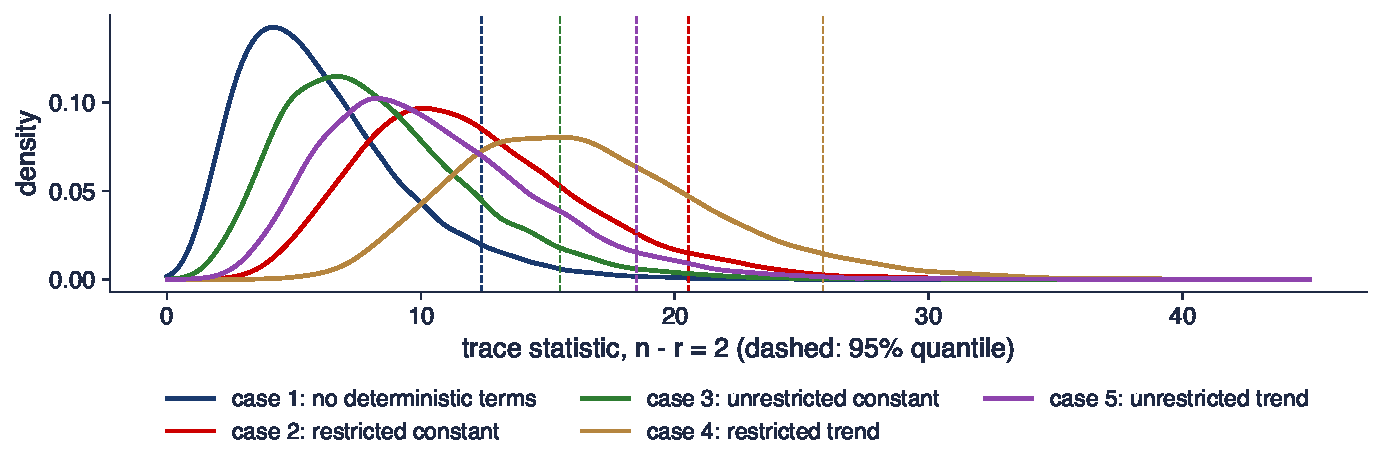
\includegraphics[width=0.97\textwidth,height=0.5\textheight,keepaspectratio]{ats_ch4_trace_dists.pdf}
\end{center}
\vspace{-0.25cm}
\begin{itemize}
    \item Trace statistic under $H(r)$ with $n - r = 2$, simulated from random walks (10\,000 replications, $T = 400$; drift in cases 3 and 5)
    \item 95\% quantiles: 12.38 (case 1), 20.53 (2), 15.48 (3), 25.84 (4), 18.50 (5)
\end{itemize}
\quantlet{ATS\_ch4\_johansen\_asymptotics}{\qlurl{ATS_ch4_johansen_asymptotics}}
\end{frame}

\begin{frame}{Interpreting the five distributions}
\itemsize{\small}
\begin{itemize}
    \item Each restricted deterministic term adds a regressor to the reduced-rank problem and shifts the distribution to the right
    \item A trend in the levels (cases 3 and 5) makes one direction of the common trend deterministic: for $n - r = 1$ the limit is $\chi^2(1)$, 95\% quantile 3.89
    \item Using case-3 critical values in a case-2 model over-rejects: the 95\% quantile for $n - r = 1$ is 9.25 in case 2 and 3.89 in case 3
    \item Our simulated quantiles differ from the published tables \refMHM\ by a few tenths at most; the Quantlet gives all cases and $n - r = 1, \dots, 4$
\end{itemize}
\end{frame}

\begin{frame}{Simulated 95\% quantiles of the trace statistic}
\itemsize{\small}
\begin{center}
\footnotesize
\begin{tabular}{lccccc}
\toprule
$n - r$ & case 1 & case 2 & case 3 & case 4 & case 5 \\
\midrule
1 & 4.21 & 9.25 & 3.89 & 12.58 & 3.84 \\
2 & 12.38 & 20.53 & 15.48 & 25.84 & 18.50 \\
3 & 24.44 & 35.24 & 29.78 & 43.14 & 35.36 \\
4 & 40.29 & 53.68 & 47.98 & 63.85 & 55.54 \\
\bottomrule
\end{tabular}
\end{center}
\begin{itemize}
    \item Simulated with 10\,000 replications of a VAR(1) test regression on $T = 400$ observations; the response-surface critical values of \refMHM\ differ by at most a few tenths
    \item Choosing the case: plot the data first; if unsure between 2 and 3 (or 3 and 4), test the joint hypothesis on rank and case in the order of the Pantula principle \refPan, \refJohC
    \item Breaks in the deterministic terms shift the distribution again: use the critical values of \refJMN\ for broken trends
\end{itemize}
\end{frame}

\begin{frame}{Recap: Deterministic terms}
\itemsize{\small}
\begin{itemize}
    \item Split each deterministic term into an $\alpha$ part (in the relations) and an $\alpha_\perp$ part (in the levels)
    \item The five cases have five different null distributions; mixing them up changes the rank
    \item Plot the data, choose the case on economic grounds and use the Pantula principle when in doubt
\end{itemize}
\end{frame}


%=============================================================================
\section{Small samples: corrections and the bootstrap}
%=============================================================================

\begin{frame}{Over-rejection of the asymptotic test}
\itemsize{\small}
\begin{itemize}
    \item The trace statistic estimates $n^2(p - 1)$ short-run parameters plus the deterministic terms; with $T = 100$ and $n = 3$, $p = 4$ this is a large share of the information
    \item The distortion grows with persistent short-run dynamics ($\Gamma_i$ near the unit circle) and with roots of the stationary part near one
    \item Three remedies
    \begin{itemize}
        \item \textbf{Reinsel--Ahn}: multiply the statistic by $(T - np)/T$ \refRA; simple, often too conservative
        \item \textbf{Bartlett correction}: $LR_{tr}/(1 + a(\theta)/T)$ with $\E LR_{tr} \approx f\,(1 + a(\theta)/T)$ \refJohG; $f$: the mean of the limit distribution; $a(\theta)$: an analytic function of the parameters $\theta$, estimated by plug-in
        \item \textbf{Bootstrap}: simulate the null distribution from the model estimated under $H(r)$ \refSwe, \refCRT
    \end{itemize}
    \item Conditional heteroskedasticity leaves the limit distribution unchanged but worsens the finite-sample size \refCRTa: use the wild bootstrap
\end{itemize}
\end{frame}

\begin{frame}{The bootstrap rank test, step by step}
\itemsize{\small}
\begin{itemize}
    \item 1. Estimate the VECM under $H(r)$: $\hat\alpha^{(r)}, \hat\beta^{(r)}, \hat\Gamma_i^{(r)}, \hat\Phi^{(r)}$ and residuals $\hat\varepsilon_t^{(r)}$
    \item 2. Generate $\Delta y_t^* = \hat\alpha^{(r)}\hat\beta^{(r)\prime}y_{t-1}^* + \sum_i\hat\Gamma_i^{(r)}\Delta y_{t-i}^* + \hat\Phi^{(r)}D_t + \varepsilon_t^*$ from the observed initial values
    \item 3. Innovations: $\varepsilon_t^* = \hat\varepsilon_t^{(r)}w_t$, $w_t \sim$ i.i.d. $N(0, 1)$ (wild) or resampled residuals (i.i.d. bootstrap)
    \begin{itemize}
        \item the star marks bootstrap quantities; $w_t$: a random sign-and-scale weight; the wild version keeps the volatility pattern of each date
    \end{itemize}
    \item 4. Compute $LR_{tr}^*(r)$ on each sample; p-value = share of $LR_{tr}^* \ge LR_{tr}(r)$; test $r = 0, 1, \dots$ and stop at the first non-rejection
    \item Estimating under $H(r)$ (not under $H(n)$) is essential: the bootstrap data must have exactly $n - r$ unit roots \refCRT
\end{itemize}
\end{frame}

\begin{frame}{Size of the rank test in small samples (simulation)}
\itemsize{\footnotesize}
\begin{center}
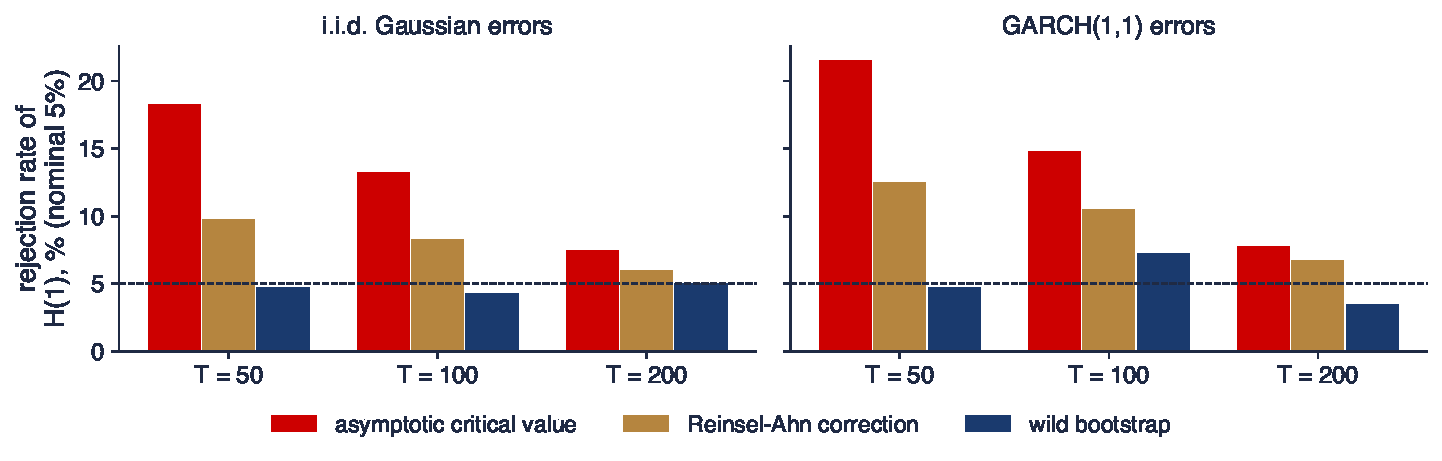
\includegraphics[width=0.97\textwidth,height=0.5\textheight,keepaspectratio]{ats_ch4_size_mc.pdf}
\end{center}
\vspace{-0.25cm}
\begin{itemize}
    \item Three-variable VECM, true rank 1, $\Gamma_1 = 0.8I$, case 2, VAR(2); test of $H(1)$ at 5\%; 400 replications, 199 bootstrap samples each
    \item $T = 50$, i.i.d. errors: asymptotic 18.2\%, Reinsel--Ahn 9.8\%, wild bootstrap 4.8\%
\end{itemize}
\quantlet{ATS\_ch4\_johansen\_asymptotics}{\qlurl{ATS_ch4_johansen_asymptotics}}
\end{frame}

\begin{frame}{Interpreting the size simulation}
\itemsize{\small}
\begin{itemize}
    \item With persistent short-run dynamics the asymptotic test finds a spurious second relation in 18.2\% of samples of 50 and 13.2\% of samples of 100
    \item Reinsel--Ahn halves the distortion; the wild bootstrap is close to 5\% at every $T$, also under GARCH errors (4.8\% at $T = 50$, asymptotic 21.5\%)
    \item At $T = 200$ all three are acceptable: the problem is the ratio of parameters to observations, not the method
    \item Practice: report asymptotic and bootstrap $p$-values side by side, and the rank for neighbouring lag lengths
\end{itemize}
\end{frame}

\begin{frame}{Recap: Small samples}
\itemsize{\small}
\begin{itemize}
    \item The asymptotic trace test over-rejects when parameters are many and the short run is persistent
    \item Reinsel--Ahn and the Bartlett correction rescale the statistic; the bootstrap rebuilds its distribution
    \item Bootstrap from the model estimated under $H(r)$; use wild weights when volatility changes over time
\end{itemize}
\end{frame}


%=============================================================================
\section{Identification and tests on $\beta$ and $\alpha$}
%=============================================================================

\begin{frame}{Normalisation is not identification (1/2)}
\itemsize{\small}
\begin{itemize}
    \item The eigenvectors give one basis of the cointegration space $\mathrm{sp}(\beta)$; any $\beta\xi$ spans the same space and fits equally well
    \begin{itemize}
        \item $\mathrm{sp}(\beta)$: the space spanned by the columns of $\beta$; $\xi$: an invertible $r\times r$ matrix (a rotation)
    \end{itemize}
    \item Dividing each vector by one coefficient fixes the scale ($r$ restrictions), but not the rotation
    \begin{itemize}
        \item $r(r - 1)$ further restrictions are needed, $r - 1$ per vector
    \end{itemize}
    \item Identification rests on economic theory: each restriction is a statement such as ``the lending rate does not depend on the deposit rate in the long run''
\end{itemize}
\end{frame}

\begin{frame}{Normalisation is not identification (2/2)}
\itemsize{\small}
\begin{itemize}
    \item Linear restrictions vector by vector: $\beta = (H_1\varphi_1, \dots, H_r\varphi_r)$
    \begin{itemize}
        \item $n_1$: the length of each vector ($n$ plus the restricted deterministic terms)
        \item $H_i$ ($n_1\times s_i$, known): the design matrix of vector $i$; $\varphi_i$ ($s_i\times 1$): its $s_i$ free coefficients
        \item $R_i = H_{i\perp}$: the restrictions written as $R_i'\beta_i = 0$
    \end{itemize}
    \item Rank condition \refJohE: for every $i$ and every set of $k$ other vectors $i_1, \dots, i_k$
    \begin{itemize}
        \item $\mathrm{rank}(R_i'(H_{i_1}, \dots, H_{i_k})) \ge k$, $k = 1, \dots, r - 1$
        \item meaning: no combination of other vectors satisfies the restrictions of vector $i$
        \item the cointegration analogue of the rank condition in simultaneous equations; the order condition alone is not enough
    \end{itemize}
\end{itemize}
\end{frame}

\begin{frame}{Testing restrictions on $\beta$ (1/2)}
\itemsize{\small}
\begin{itemize}
    \item \textbf{The same restriction on all vectors}, $\beta = H\varphi$: solve $|\lambda H'S_{11}H - H'S_{10}S_{00}^{-1}S_{01}H| = 0$
    \begin{itemize}
        \item $H$ ($n_1\times s$, known): the restriction; $\varphi$ ($s\times r$): the free coefficients; e.g.\ excluding one variable from all relations
        \item $\tilde\lambda_i$: the eigenvalues of the restricted problem; $\hat\lambda_i$: the unrestricted ones
    \end{itemize}
    \item Test statistic: $LR = T\sum_{i=1}^r\ln\{(1 - \tilde\lambda_i)/(1 - \hat\lambda_i)\} \to \chi^2(r(n_1 - s))$
    \begin{itemize}
        \item $LR \ge 0$; it is large when the restriction lowers the canonical correlations, i.e.\ when the data reject it
        \item degrees of freedom $r(n_1 - s)$: $n_1 - s$ restrictions on each of the $r$ vectors
    \end{itemize}
    \item Given the rank, $\hat\beta$ is super-consistent and mixed Gaussian: LR tests on $\beta$ are $\chi^2$, unlike the rank test \refJohB
\end{itemize}
\end{frame}

\begin{frame}{Testing restrictions on $\beta$ (2/2)}
\itemsize{\small}
\begin{itemize}
    \item \textbf{Different restrictions per vector}, $\beta = (H_1\varphi_1, \dots, H_r\varphi_r)$: no closed form
    \begin{itemize}
        \item maximise the concentrated log-likelihood $-\tfrac{T}{2}\ln|\hat\Omega(\beta)|$ by the switching algorithm (one vector at a time) or numerically
        \item over-identifying restrictions: $LR \to \chi^2(\sum_i(n_1 - r + 1 - s_i))$; each vector has $n_1 - r + 1 - s_i$ restrictions beyond the $r - 1$ needed to identify it
    \end{itemize}
    \item \textbf{Fully known} $\beta = \beta_0$ (e.g.\ the great ratios): \[ LR = T\Big\{\ln|\hat\Omega(\beta_0)| - \ln|S_{00}| - \sum_{i\le r}\ln(1 - \hat\lambda_i)\Big\} \to \chi^2(r(n_1 - r)) \]
    \begin{itemize}
        \item compares the fit with $\beta_0$ imposed ($\hat\Omega(\beta_0)$) to the unrestricted fit; $\beta_0$: the hypothesised matrix
    \end{itemize}
\end{itemize}
\end{frame}

\begin{frame}{Restrictions on $\alpha$ and weak exogeneity}
\itemsize{\small}
\begin{itemize}
    \item $\alpha = A\psi$: only $m$ combinations of the equations adjust to the relations
    \begin{itemize}
        \item $A$ ($n\times m$, known): the restriction; $\psi$ ($m\times r$): the free adjustment coefficients; $A_\perp$: its orthogonal complement
        \item condition the system on $A_\perp'R_{0t}$ and solve the eigenvalue problem of the remaining $m$ equations (eigenvalues $\tilde\lambda_i$)
        \item $LR = T\sum_{i\le r}\ln\{(1 - \tilde\lambda_i)/(1 - \hat\lambda_i)\} \to \chi^2(r(n - m))$
    \end{itemize}
    \item \textbf{Weak exogeneity} of $x_t$ for $\beta$: the row of $\alpha$ for $x_t$ is zero (a zero row of $\alpha$, $r$ restrictions)
    \begin{itemize}
        \item $x_t$ does not adjust to past disequilibria; it is a common trend (a column of $\alpha_\perp$)
        \item the conditional model of $\Delta y_t$ given $\Delta x_t$ is then fully efficient for $\beta$: the basis of single-equation ECM and ARDL
    \end{itemize}
    \item Long-run structural hypotheses are joint restrictions on $\beta$ and $\alpha$
    \begin{itemize}
        \item PPP: $(1, -1, -1)$ on (price, foreign price, exchange rate); Fisher: $(1, -1)$ on (interest rate, inflation); complete pass-through: $(1, -1)$ on (retail rate, policy or market rate)
    \end{itemize}
\end{itemize}
\end{frame}

\begin{frame}{Recap: Identification and tests}
\itemsize{\small}
\begin{itemize}
    \item Identify $\beta$ with $r - 1$ economically motivated restrictions per vector; check the rank condition
    \item Given the rank, LR tests on $\beta$ and $\alpha$ are $\chi^2$ with known degrees of freedom
    \item A zero row of $\alpha$ = weak exogeneity = permission to condition on that variable
\end{itemize}
\end{frame}


%=============================================================================
\section{Application: interest-rate pass-through in Romania}
%=============================================================================

\begin{frame}{How fast and how fully do banks follow ROBOR?}
\itemsize{\footnotesize}
\begin{columns}[T]
\begin{column}{0.36\textwidth}
\centering

\includegraphics[height=0.34\textheight]{ch0_bnr_palace_2015.jpg}\\[1mm]
\imgcap{The BNR palace, Bucharest}
\imgcredit{https://commons.wikimedia.org/wiki/File:Bucharest_-_BNR_Palace_(19644434340).jpg}{Photo: Ștefan Jurcă (2015); CC BY 2.0; Wikimedia Commons}
\end{column}
\begin{column}{0.62\textwidth}
\begin{itemize}
    \item Monetary policy reaches households and firms only through bank rates; ROBOR 3M is the reference for most variable-rate loans in lei
    \item Euro area: long-run pass-through to lending rates often complete, to deposit rates incomplete \refdB; CEE: faster and fuller pass-through after the early transition \refECR
    \item Hypotheses: $H_\beta$: lending and deposit rates move one for one with ROBOR in the long run; $H_\alpha$: ROBOR does not adjust to bank rates
    \item Data: August 2005 -- March 2026, $T = 248$ months (inflation targeting)
\end{itemize}
\end{column}
\end{columns}
\end{frame}

\begin{frame}{Lending rate, deposit rate and ROBOR 3M}
\itemsize{\footnotesize}
\begin{center}
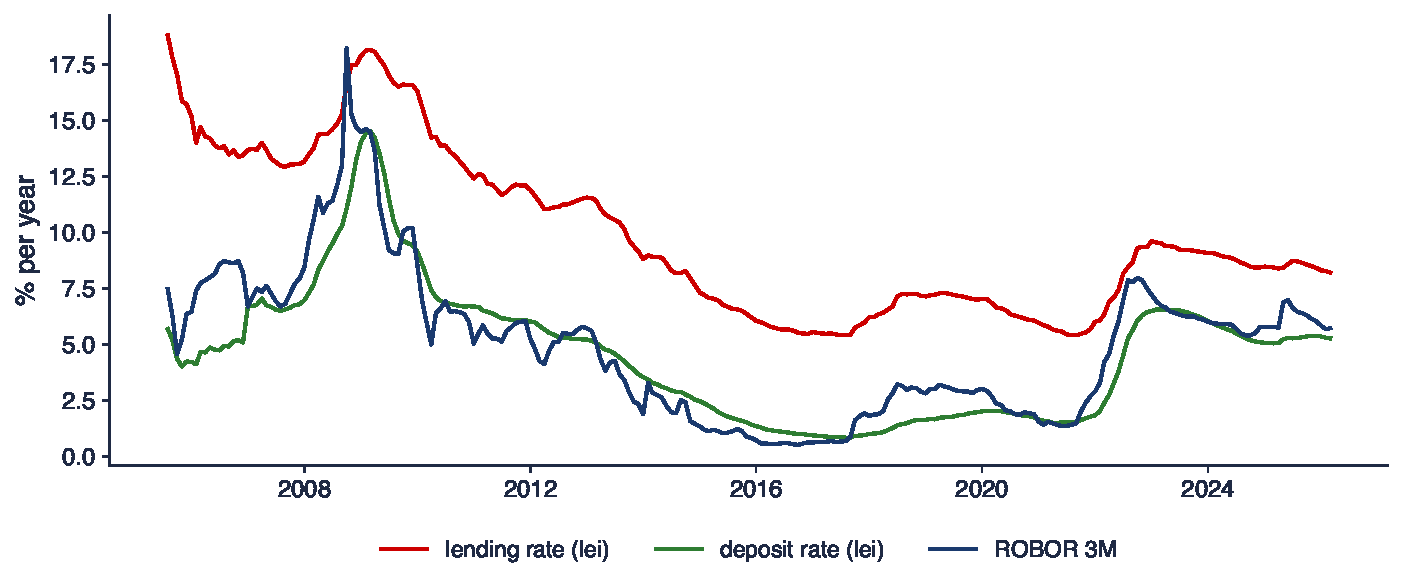
\includegraphics[width=0.97\textwidth,height=0.5\textheight,keepaspectratio]{ats_ch4_rates.pdf}
\end{center}
\vspace{-0.25cm}
\begin{itemize}
    \item Monthly, \% per year; lending and deposit rates in lei (IMF IFS, reported by the BNR); ROBOR 3M (Eurostat)
    \item ROBOR ranges from 0.51\% to 18.2\%; the lending--ROBOR spread falls from 11.3 pp to 2.5 pp
\end{itemize}
\quantlet{ATS\_ch4\_passthrough\_vecm}{\qlurl{ATS_ch4_passthrough_vecm}}
\end{frame}

\begin{frame}{Interpreting the three rates}
\itemsize{\small}
\begin{itemize}
    \item All three rates wander far from any mean over twenty years: treat them as I(1) within the sample, even if interest rates are bounded in theory
    \item They move together after 2008, in 2014--2015 and in 2022: the visual case for cointegration
    \item The falling spread in 2005--2010 is the end of the transition (competition, falling risk premia), not a policy effect
    \item No trend in levels is plausible for rates: case 2, constant restricted to the relations
\end{itemize}
\end{frame}

\begin{frame}{Rank of the pass-through system}
\itemsize{\small}
\begin{center}
\scriptsize
\begin{tabular}{lccccccc}
\toprule
$H(r)$ & $LR_{tr}$ & RA & cv 5\% & wild $p$ & $LR_{tr}$, $p{=}4$ & RA, $p{=}4$ & wild $p$, $p{=}4$ \\
\midrule
$r = 0$ & 121.1 & 118.1 & 35.2 & 0.007 & 40.0 & 38.0 & 0.647 \\
$r \le 1$ & 52.2 & 50.9 & 20.5 & 0.022 & 14.9 & 14.1 & 0.812 \\
$r \le 2$ & 4.3 & 4.2 & 9.3 & 0.767 & 3.8 & 3.6 & 0.820 \\
\bottomrule
\end{tabular}
\end{center}
\begin{itemize}
    \item Case 2; RA: Reinsel--Ahn; cv: simulated 95\% quantile; wild $p$: 399 wild-bootstrap samples under $H(r)$; lag order by BIC = 2, HQ = 5, AIC = 8
    \item With $p = 2$ all three methods give $r = 2$; with $p = 4$ the asymptotic test gives $r = 1$ and the wild bootstrap rejects nothing
\end{itemize}
\end{frame}

\begin{frame}{Interpreting the rank tests}
\itemsize{\small}
\begin{itemize}
    \item Two relations are what theory predicts: one for lending rates, one for deposit rates, both anchored to ROBOR
    \item The result is fragile: two extra lags and heteroskedasticity-robust inference remove the evidence; the 2008--2009 volatility dominates the sample
    \item We continue with $r = 2$ because theory and the parsimonious model agree, and we report the sensitivity
    \item A rank chosen this way is a modelling decision, not a measurement: state it before testing restrictions
\end{itemize}
\end{frame}

\begin{frame}{Identified relations and the tests}
\itemsize{\small}
\begin{itemize}
    \item Just-identified (one exclusion per vector): $\text{lend}_t = 1.13\,\text{ROBOR}_t + 3.62$, $\text{dep}_t = 0.93\,\text{ROBOR}_t + 0.09$
    \item Adjustment: lending rate $\alpha_{11} = \ensuremath{-}0.056$ (to its own relation), deposit rate $\alpha_{22} = \ensuremath{-}0.071$; ROBOR: 0.014 and 0.017
    \item \begin{center}
\scriptsize
\begin{tabular}{lccc}
\toprule
\textbf{Hypothesis} & $LR$ & df & $p$ \\
\midrule
complete pass-through to both rates & 8.98 & 2 & 0.011 \\
complete pass-through to the lending rate & 4.16 & 1 & 0.041 \\
ROBOR weakly exogenous (zero row of $\alpha$) & 0.57 & 2 & 0.752 \\
\bottomrule
\end{tabular}
\end{center}

    \item With $p = 4$: lending pass-through 1.11, $p$-value of complete pass-through to lending 0.458, of weak exogeneity 0.819
\end{itemize}
\end{frame}

\begin{frame}{The two equilibrium errors}
\itemsize{\footnotesize}
\begin{center}
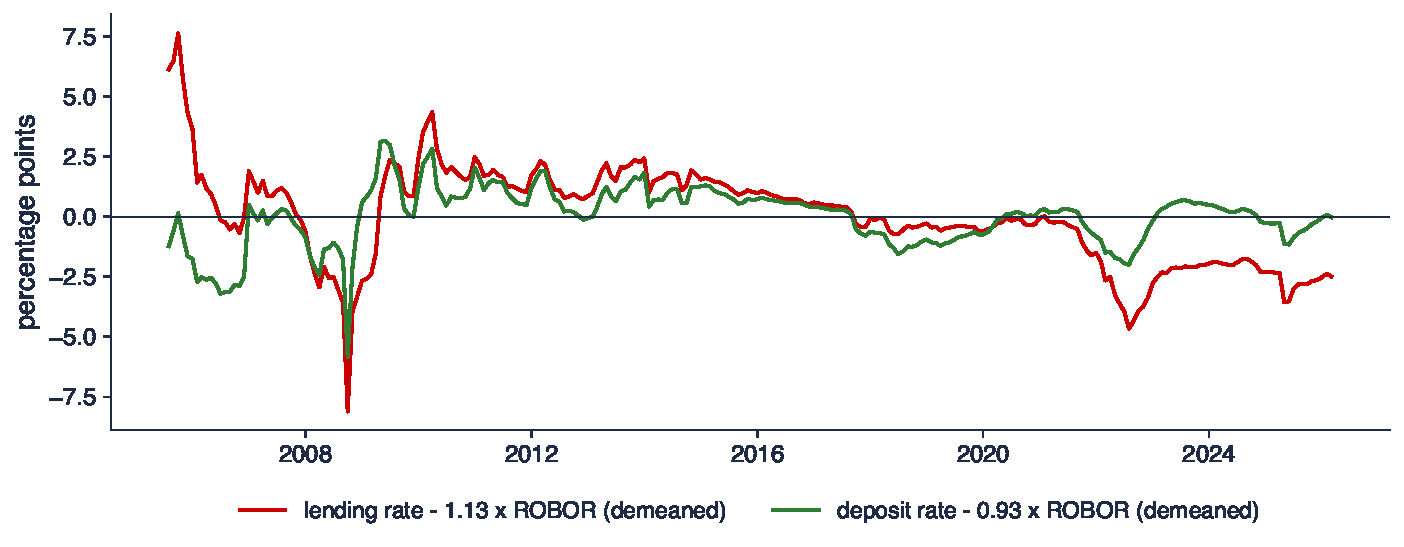
\includegraphics[width=0.97\textwidth,height=0.52\textheight,keepaspectratio]{ats_ch4_pt_ect.pdf}
\end{center}
\vspace{-0.25cm}
\begin{itemize}
    \item $\hat\beta_i'y_t$ for the just-identified relations, demeaned; they should look stationary if the rank and $\beta$ are right
\end{itemize}
\quantlet{ATS\_ch4\_passthrough\_vecm}{\qlurl{ATS_ch4_passthrough_vecm}}
\end{frame}

\begin{frame}{Interpreting the pass-through VECM}
\itemsize{\small}
\begin{itemize}
    \item Lending rates over-react slightly in the long run (1.13 per point of ROBOR), deposit rates under-react (0.93): the bank margin widens when ROBOR rises
    \item Joint complete pass-through is rejected ($p = 0.011$), driven by deposits; for lending rates alone the verdict depends on the lag length
    \item ROBOR is weakly exogenous ($p = 0.752$): money-market rates lead, bank rates follow; this justifies a single-equation ARDL
    \item The lending equilibrium error is persistent before 2010: the transition-era spread is not a stable markup, a candidate for a broken constant \refJMN
\end{itemize}
\end{frame}

\begin{frame}{Recap: Pass-through in Romania}
\itemsize{\small}
\begin{itemize}
    \item Two cointegrating relations with ROBOR as the common trend, but the rank is sensitive to lags and to heteroskedasticity
    \item Lending pass-through close to (slightly above) one, deposit pass-through below one
    \item Weak exogeneity of ROBOR is not rejected: a conditional single-equation model is legitimate
\end{itemize}
\end{frame}


%=============================================================================
\section{I(2) in brief}
%=============================================================================

\begin{frame}{When the I(1) model is not enough}
\itemsize{\small}
\begin{itemize}
    \item If $\alpha_\perp'\Gamma\beta_\perp$ has reduced rank $s < n - r$, the Granger representation fails: some common trends are I(2), $y_t$ contains $\sum\sum\varepsilon$
    \item Typical candidates: nominal price levels and nominal money in periods of changing inflation; inflation is then I(1)
    \item I(2) model: two reduced-rank conditions, $\Pi = \alpha\beta'$ and $\alpha_\perp'\Gamma\beta_\perp = \xi\eta'$; ML and rank tests in \refJohF, applied guidance in \refJus
    \begin{itemize}
        \item polynomial cointegration: $\beta'y_t + \delta'\Delta y_t \sim$ I(0), e.g.\ real money plus a multiple of inflation
    \end{itemize}
    \item Practical check: test $\Delta y_t$ for a unit root; if the I(1) VECM has a root near one in the stationary part, suspect I(2); the usual fix is to model real (deflated) variables
\end{itemize}
\end{frame}

\begin{frame}{Is the Romanian price level I(2)?}
\itemsize{\footnotesize}
\begin{center}
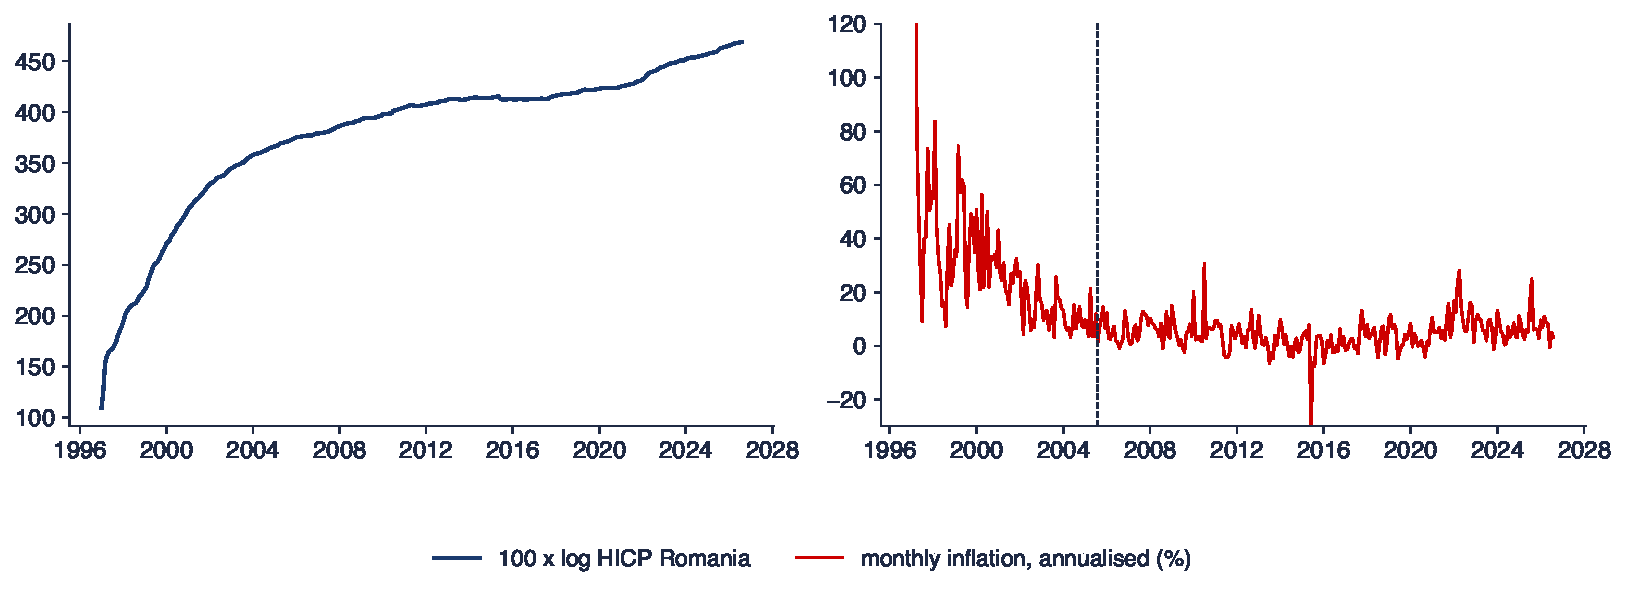
\includegraphics[width=0.97\textwidth,height=0.48\textheight,keepaspectratio]{ats_ch4_i2.pdf}
\end{center}
\vspace{-0.25cm}
\begin{itemize}
    \item Left: $100\ln$ HICP; right: monthly inflation, annualised; dashed line: inflation targeting from August 2005
    \item ADF $t$ on monthly inflation (12 lags): \ensuremath{-}4.25 for 1997--2026, \ensuremath{-}2.39 since 2005 (5\% critical value $-2.87$); on its change: \ensuremath{-}6.13
\end{itemize}
\quantlet{ATS\_ch4\_i2\_check}{\qlurl{ATS_ch4_i2_check}}
\end{frame}

\begin{frame}{Interpreting the I(2) check}
\itemsize{\small}
\begin{itemize}
    \item Over 1997--2026, disinflation looks like mean reversion and inflation tests as stationary: the price level is I(1)
    \item Since 2005 a unit root in inflation is not rejected: within the inflation-targeting sample the price level behaves like I(2)
    \item The answer depends on the sample, as for the rank: this is why systems with nominal levels are usually rewritten in real terms and inflation
    \item Our pass-through system uses rates, which are at most I(1): the I(2) issue does not arise there
\end{itemize}
\end{frame}


%=============================================================================
\section{Structural VECM: common trends}
%=============================================================================

\begin{frame}{Permanent and transitory shocks (1/2)}
\itemsize{\small}
\begin{itemize}
    \item Granger representation: the long-run effect of $\varepsilon_t$ on $y_{t+h}$, $h \to \infty$, is $C\varepsilon_t$, and $\mathrm{rank}\,C = n - r$
    \item Structural shocks: $\varepsilon_t = Bu_t$, $\E u_tu_t' = I$
    \begin{itemize}
        \item $u_t$: $n$ uncorrelated shocks with unit variance; $B$ ($n\times n$): their impact effects, $BB' = \Omega$
        \item the long-run impact $CB$ has at most $n - r$ non-zero columns: $k = n - r$ permanent and $r$ transitory shocks
    \end{itemize}
    \item Counting (\atschlink{https://danpele.github.io/Advanced-Time-Series/EN/Courses/chapter3_structural_var_local_projections.pdf}{Chapter 3} needed $n(n - 1)/2$ restrictions): cointegration gives $rk$ zero long-run restrictions for free
    \begin{itemize}
        \item still needed: $k(k - 1)/2$ among the permanent shocks and $r(r - 1)/2$ among the transitory shocks \refKL, \refGN
    \end{itemize}
\end{itemize}
\end{frame}

\begin{frame}{Permanent and transitory shocks (2/2)}
\itemsize{\small}
\begin{itemize}
    \item With one common trend ($k = 1$) the permanent shock is identified without further assumptions
    \begin{itemize}
        \item the shock: $u_t^P = \alpha_\perp'\varepsilon_t/(\alpha_\perp'\Omega\alpha_\perp)^{1/2}$, the innovation of the common trend scaled to unit variance
        \item its impact: $b^P = \Omega\alpha_\perp(\alpha_\perp'\Omega\alpha_\perp)^{-1/2}$, the column of $B$ that moves the $n$ variables on impact
    \end{itemize}
    \item This generalises Blanchard--Quah (\atschlink{https://danpele.github.io/Advanced-Time-Series/EN/Courses/chapter3_structural_var_local_projections.pdf}{Chapter 3}): there the long-run zero was imposed; here it comes from the cointegration rank
\end{itemize}
\end{frame}

\begin{frame}{Case study: King, Plosser, Stock and Watson (1991)}
\itemsize{\small}
\begin{itemize}
    \item \refKPSW: in a real business-cycle model with a stochastic productivity trend, consumption, investment and output share one trend: the great ratios $c - y$ and $i - y$ are stationary
    \begin{itemize}
        \item $n = 3$, $r = 2$, $\beta = \begin{pmatrix}1 & 0\\ 0 & 1\\ -1 & -1\end{pmatrix}$ imposed; one permanent ``balanced-growth'' shock
        \item question: how much of the business cycle does the permanent shock explain?
    \end{itemize}
    \item Our replication: US quarterly 1949Q1--1988Q4 (the paper's sample), $T = 160$; $c$: nondurables and services, $i$: fixed investment, $y$: GDP, per capita, deflated by the GDP deflator
    \begin{itemize}
        \item VAR($2$) in levels (all criteria), case 3; trace: 45.8, 19.4, 1.4 against 95\% quantiles 29.8, 15.5, 3.9: $r = 2$
        \item the exact great ratios are rejected: $LR = 16.6$, $\chi^2(2)$, $p = $<$\,0.001$; with a restricted trend (case 4) they are not: $LR = 0.50$, $p = 0.778$
    \end{itemize}
\end{itemize}
\end{frame}

\begin{frame}{The balanced-growth shock}
\itemsize{\footnotesize}
\begin{center}
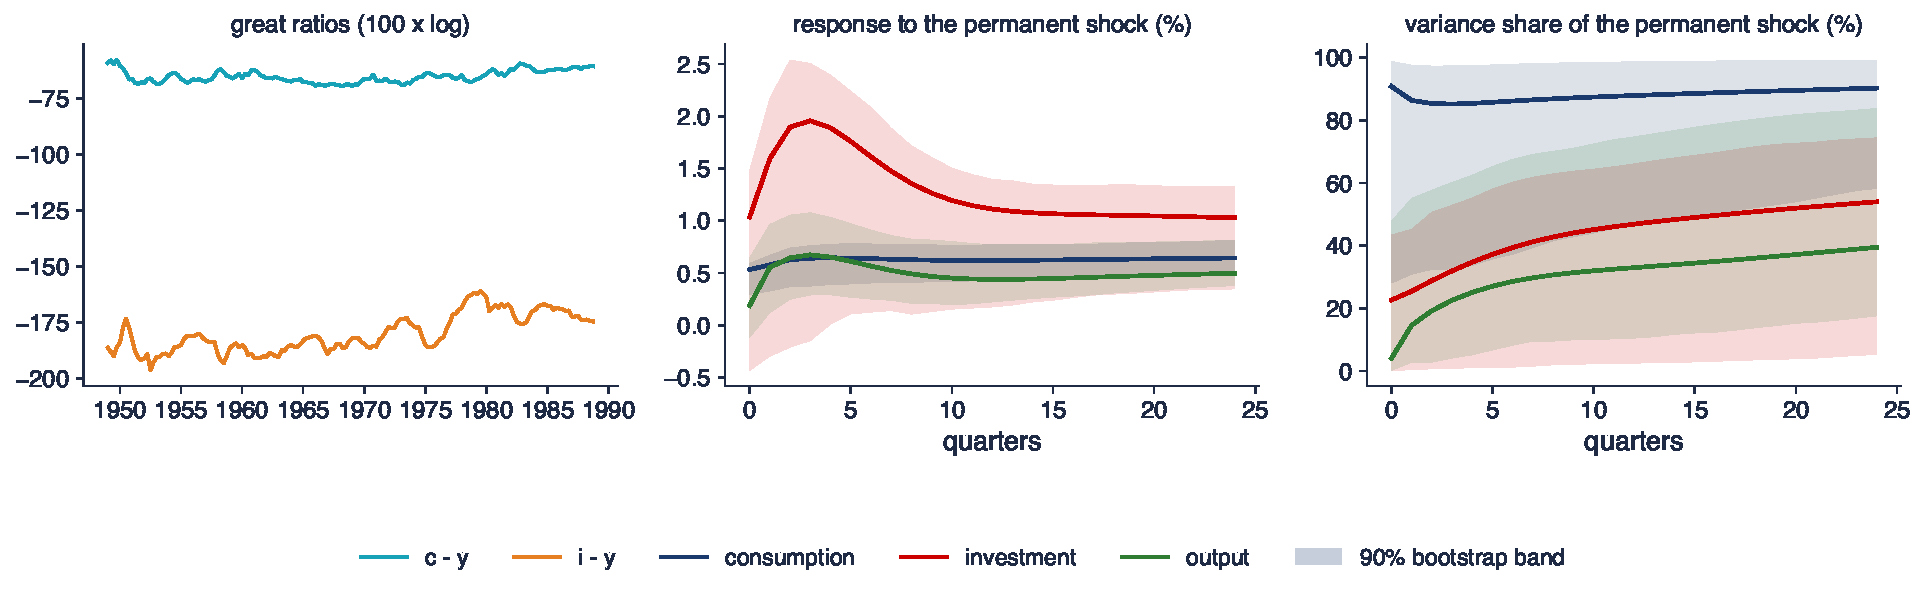
\includegraphics[width=0.97\textwidth,height=0.48\textheight,keepaspectratio]{ats_ch4_kpsw.pdf}
\end{center}
\vspace{-0.25cm}
\begin{itemize}
    \item Great ratios imposed (case 3); one-standard-deviation permanent shock; 90\% residual-bootstrap bands (300 samples, $\beta$ fixed)
    \item Long-run effect 0.74\% on all three; share in output variance: 4\% at 1 quarter, 30\% at 8, 39\% at 24 [17; 83]
\end{itemize}
\quantlet{ATS\_ch4\_common\_trends}{\qlurl{ATS_ch4_common_trends}}
\end{frame}

\begin{frame}{Interpreting the common-trends model}
\itemsize{\small}
\begin{itemize}
    \item Balanced growth holds by construction in the long run: the shock moves $c$, $i$ and $y$ by the same 0.74\%; investment overshoots in the short run
    \item The permanent shock dominates consumption (87\% at 8 quarters, the permanent-income logic) but explains a minority of output fluctuations at business-cycle horizons
    \item Bands are wide: with $T = 160$ the data barely separate permanent from transitory variation
    \item As in \atschlink{https://danpele.github.io/Advanced-Time-Series/EN/Courses/chapter3_structural_var_local_projections.pdf}{Chapter 3}, the economics is in the identifying assumption: here, which relations are stationary
\end{itemize}
\end{frame}

\begin{frame}{How robust is the answer?}
\itemsize{\small}
\begin{center}
\footnotesize
\begin{tabular}{lcccc}
\toprule
\textbf{Specification} & $h = 1$ & $h = 4$ & $h = 8$ & $h = 24$ \\
\midrule
great ratios, case 3, 1949--1988 & 4\% & 23\% & 30\% & 39\% \\
great ratios with trend, case 4, 1949--1988 & 34\% & 37\% & 52\% & 77\% \\
great ratios, case 3, 1949--2019 & 51\% & 30\% & 29\% & 40\% \\
great ratios, case 3, 1949--2025 & 28\% & 20\% & 20\% & 29\% \\
\bottomrule
\end{tabular}
\end{center}
\begin{itemize}
    \item Share of the permanent shock in the forecast error variance of output, $h$ quarters ahead
    \item Allowing the ratios to trend (services gaining share) raises the role of the permanent shock considerably at short horizons; extending the sample changes it again; the great-ratio LR rises to 24.3 on data to 2025
    \item Conclusion: the size of ``trend shocks'' in the cycle is not pinned down by the data alone
\end{itemize}
\end{frame}

\begin{frame}{Recap: Structural VECM}
\itemsize{\small}
\begin{itemize}
    \item Cointegration splits shocks into $n - r$ permanent and $r$ transitory ones and supplies $rk$ long-run zeros
    \item With one common trend the permanent shock is $\alpha_\perp'\varepsilon_t$, scaled
    \item KPSW: balanced growth gives a clean identification, but the variance shares depend on the deterministic case and the sample
\end{itemize}
\end{frame}


%=============================================================================
\section{ARDL and the bounds test}
%=============================================================================

\begin{frame}{From a VECM to a conditional ECM (1/2)}
\itemsize{\small}
\begin{itemize}
    \item Partition $y_t = (y_t, x_t')'$, $x_t$ of dimension $k$; if $x_t$ is weakly exogenous and there is one relation involving $y_t$, the conditional model is \[ \Delta y_t = c_0 + c_1t + \pi_{yy}y_{t-1} + \pi_{yx}'x_{t-1} + \sum_{i=1}^{p-1}\psi_i\Delta y_{t-i} + \sum_{j=0}^{q-1}\omega_j'\Delta x_{t-j} + u_t \]
    \item Notation \refPSSb
    \begin{itemize}
        \item $y_t$: the dependent variable; $x_t$: the $k$ forcing variables; $c_0$, $c_1$: intercept and trend coefficient
        \item $\pi_{yy}$ (scalar), $\pi_{yx}$ ($k\times 1$): the coefficients on the lagged levels, i.e.\ the long-run part
        \item $\psi_i$, $\omega_j$: short-run coefficients; $p$, $q$: lag orders; $u_t$: the error, uncorrelated with $\Delta x_t$
    \end{itemize}
\end{itemize}
\end{frame}

\begin{frame}{From a VECM to a conditional ECM (2/2)}
\itemsize{\small}
\begin{itemize}
    \item This is an ARDL($p, q$) in levels, rewritten
    \begin{itemize}
        \item long-run coefficients $\theta = -\pi_{yx}/\pi_{yy}$: the equilibrium is $y = \theta'x$ (plus constant)
        \item speed of adjustment $\pi_{yy} \in (-1, 0)$: the share of last period's disequilibrium corrected this period; half-life $\ln 0.5/\ln(1 + \pi_{yy})$
    \end{itemize}
    \item Inference
    \begin{itemize}
        \item OLS is consistent and $\hat\theta$ has a mixed-Gaussian limit when the lags absorb the endogeneity of $x_t$ \refPSa
        \item standard errors of $\hat\theta$ by the delta method; $t$-tests on $\theta$ are asymptotically valid
    \end{itemize}
    \item The attraction: $x_t$ may be I(0), I(1) or a mix, and we need not pre-test it
\end{itemize}
\end{frame}

\begin{frame}{The bounds test}
\itemsize{\small}
\begin{itemize}
    \item $H_0$: no level relationship, $\pi_{yy} = 0$ and $\pi_{yx} = 0$; Wald $F$ (and $t$ on $\pi_{yy}$ to exclude the degenerate case $\pi_{yy} = 0 \ne \pi_{yx}$)
    \item The null distribution depends on the integration order of $x_t$: lower bound if all of $x_t$ is I(0), upper bound if all is I(1)
    \begin{itemize}
        \item $F$ above the upper bound: reject (a level relationship); below the lower bound: do not reject; between: inconclusive, then the order of integration matters
    \end{itemize}
    \item Five cases (as in Johansen): I none; II restricted intercept; III unrestricted intercept; IV unrestricted intercept, restricted trend; V unrestricted intercept and trend
    \begin{itemize}
        \item in cases II and IV the restricted terms are part of $H_0$; the $t$-bounds exist for cases I, III, V
    \end{itemize}
    \item Simulated 5\% bounds ($T = 1000$, 10\,000 replications), $k = 1$: case II [3.58; 4.14], case III [4.97; 5.71]; $t$, case III: [\ensuremath{-}2.86; \ensuremath{-}3.22]
\end{itemize}
\end{frame}

\begin{frame}{Critical values in small samples}
\itemsize{\small}
\begin{itemize}
    \item PSS tabulate asymptotic bounds ($T = 1000$); with 30--80 annual observations they are too low \refNar
    \item Our simulation, case III, $k = 1$, 5\%: $T = 30$: [5.52; 6.32], $T = 80$: [5.02; 5.86], $T = 250$: [4.98; 5.73], asymptotic: [4.97; 5.71]
    \item Response-surface regressions give critical values and approximate $p$-values for any $T$, $k$ and lag order \refKS: use them instead of the asymptotic table
    \item Frequent misuses in applied work
    \begin{itemize}
        \item the wrong case (case III bounds for a model estimated in case II); I(2) regressors, for which the bounds are invalid
        \item feedback from $y_t$ to $x_t$ (no weak exogeneity), or more than one relation among the variables
    \end{itemize}
\end{itemize}
\end{frame}

\begin{frame}{ARDL or VECM?}
\itemsize{\small}
\begin{center}
\scriptsize
\begin{tabular}{>{\raggedright\arraybackslash}p{3.0cm}>{\raggedright\arraybackslash}p{4.4cm}>{\raggedright\arraybackslash}p{4.4cm}}
\toprule
 & \textbf{ARDL} & \textbf{VECM} \\
\midrule
Relations & one, normalised on $y_t$ & $r$, rank estimated \\
Regressors & I(0), I(1) or mixed; weakly exogenous & all I(1); all endogenous \\
Inference & bounds $F$ and $t$; $\theta$ by the delta method & trace/max-eigenvalue; $\chi^2$ tests on $\beta$, $\alpha$ \\
Small samples & few parameters; small-sample bounds needed & many parameters; bootstrap needed \\
Structural use & multipliers of $x$ on $y$ & common trends, identified shocks \\
\bottomrule
\end{tabular}
\end{center}
\begin{itemize}
    \item Rule: estimate the VECM first when you can; if a variable is weakly exogenous and the relation is unique, the ARDL is efficient and simpler; if feedback is present, ARDL estimates are inconsistent
\end{itemize}
\end{frame}

\begin{frame}{ARDL pass-through of ROBOR to the lending rate}
\itemsize{\small}
\begin{itemize}
    \item ARDL(4, 2) selected by BIC, case II (ROBOR weakly exogenous in the VECM), $n = 244$
    \item Bounds $F = 4.27$; 5\% bounds asymptotic [3.58; 4.14], at our $T$ [3.67; 4.14]: a level relationship
    \begin{itemize}
        \item the same regression in case III: $F = 5.87$ against [4.94; 5.79]: inconclusive; $t = \ensuremath{-}3.28$ against [\ensuremath{-}2.86; \ensuremath{-}3.22]
    \end{itemize}
    \item Long-run pass-through $\hat\theta = 1.15$ (SE 0.12): complete pass-through not rejected by the $t$-test; speed $\hat\pi_{yy} = \ensuremath{-}0.026$ (SE 0.008), half-life 27 months
    \item Deposit rate: $F = 7.68$, $\hat\theta = 0.94$ (SE 0.05), half-life 12 months: incomplete but faster
\end{itemize}
\end{frame}

\begin{frame}{Small-sample bounds and the dynamic multipliers}
\itemsize{\footnotesize}
\begin{center}
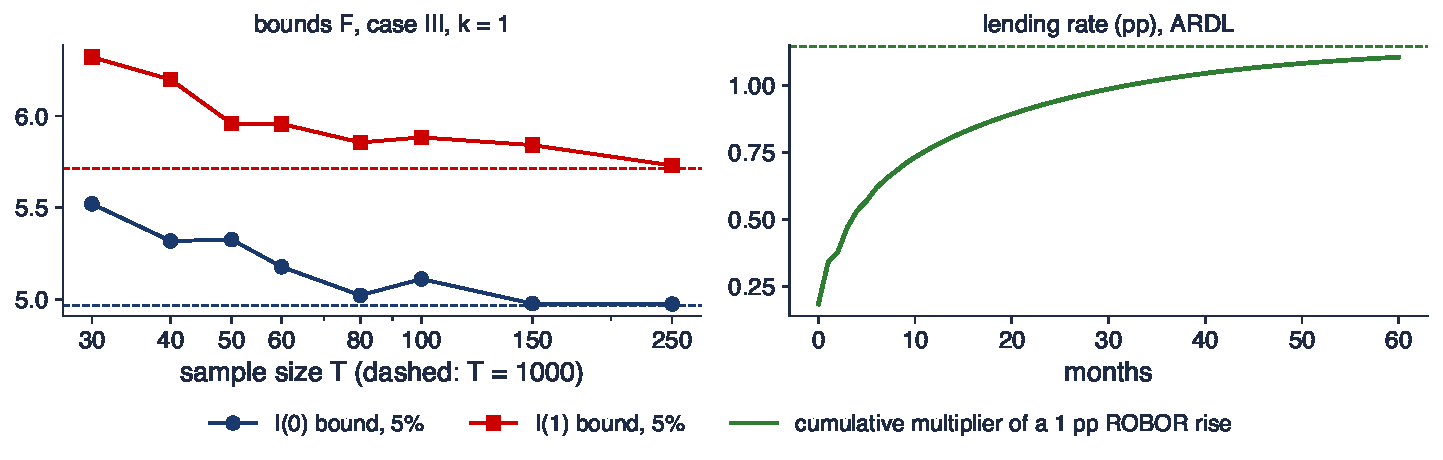
\includegraphics[width=0.97\textwidth,height=0.48\textheight,keepaspectratio]{ats_ch4_bounds.pdf}
\end{center}
\vspace{-0.25cm}
\begin{itemize}
    \item Left: simulated 5\% bounds, case III, $k = 1$, against $T$ (dashed: $T = 1000$); right: cumulative response of the lending rate to a permanent 1 pp rise of ROBOR (dashed: $\hat\theta$)
    \item Multipliers: 0.18 on impact, 0.62 after 6 months, 0.77 after 12, 0.94 after 24, 1.11 after 60
\end{itemize}
\quantlet{ATS\_ch4\_ardl\_bounds}{\qlurl{ATS_ch4_ardl_bounds}}
\end{frame}

\begin{frame}{Interpreting the ARDL results}
\itemsize{\small}
\begin{itemize}
    \item The upper bound falls from 6.32 at $T = 30$ to 5.73 at $T = 250$: with annual data the asymptotic table over-rejects
    \item The verdict on a level relationship depends on the case: decide case II or III from economics (no drift in rates) before looking at $F$
    \item ARDL and VECM agree on the size of the lending pass-through (1.15 and 1.13) but not on the test of $\theta = 1$: different nuisance parameters, different power
    \item About half of the long-run effect arrives within six months (0.62); the rest is slow, with a half-life of the disequilibrium of 27 months, consistent with fixed-rate periods and contract repricing
\end{itemize}
\end{frame}

\begin{frame}{Two related tools}
\itemsize{\small}
\begin{itemize}
    \item \textbf{Toda--Yamamoto causality} \refTY: in a VAR of possibly integrated or cointegrated variables, fit $p + d_{\max}$ lags in levels and test only the first $p$; $d_{\max}$: the highest suspected order of integration
    \begin{itemize}
        \item the Wald statistic is asymptotically $\chi^2(p)$ whatever the integration and cointegration properties; the price: lower power than a correctly specified VECM
    \end{itemize}
    \item \textbf{Nonlinear ARDL} \refSYG: split $x_t$ into partial sums of increases $x_t^+ = \sum_{j\le t}\max(\Delta x_j, 0)$ and decreases $x_t^- = \sum_{j\le t}\min(\Delta x_j, 0)$
    \begin{itemize}
        \item $x_t^+$ and $x_t^-$ enter the ARDL as two regressors, with long-run coefficients $\theta^+$, $\theta^-$ and short-run coefficients $\omega_j^+$, $\omega_j^-$
        \item long-run asymmetry: $\theta^+ \ne \theta^-$; short-run asymmetry: different $\omega_j^\pm$; Wald tests, bounds with $k = 2$
        \item classic use: retail fuel prices rise fast with oil and fall slowly (``rockets and feathers'') \refBac; Seminar 4 tests it for Romania
    \end{itemize}
\end{itemize}
\end{frame}

\begin{frame}{Recap: ARDL and the bounds test}
\itemsize{\small}
\begin{itemize}
    \item The conditional ECM is an ARDL rewritten; it needs weak exogeneity and a single relation
    \item The bounds test avoids pre-testing the regressors, at the price of an inconclusive zone
    \item Use the right case and small-sample (response-surface) critical values
    \item Toda--Yamamoto for causality without pre-testing; NARDL for asymmetric adjustment
\end{itemize}
\end{frame}


%=============================================================================
\section{Panel time series}
%=============================================================================

\begin{frame}{Panels: the gain and the new problems}
\itemsize{\footnotesize}
\begin{columns}[T]
\begin{column}{0.30\textwidth}
\centering

\includegraphics[height=0.27\textheight]{ch4_ecb_frankfurt_2015.jpg}\\[1mm]
\imgcap{The ECB seat, Frankfurt}
\imgcredit{https://commons.wikimedia.org/wiki/File:Seat_of_the_European_Central_Bank_and_Frankfurt_Skyline_at_dawn_20150422_1.jpg}{Photo: DXR (2015); CC BY-SA 4.0; Wikimedia Commons}
\end{column}
\begin{column}{0.68\textwidth}
\begin{itemize}
    \item Country series are short (20--30 years of annual data): a single-country rank or bounds test has little power; $N$ countries add information
    \item Asymptotics in two dimensions: sequential ($T \to \infty$, then $N \to \infty$) or joint with $N/T \to 0$; a panel regression of I(1) series estimates a long-run average relation even without cointegration \refPM, \refKao
    \item Two new problems: \textbf{heterogeneity} (dynamics differ across countries) and \textbf{cross-section dependence} (common shocks: the 2009 recession, COVID-19, the euro)
    \item First-generation tests assume independent units; second-generation tests model the dependence \refBrP
\end{itemize}
\end{column}
\end{columns}
\end{frame}

\begin{frame}{Measuring cross-section dependence}
\itemsize{\small}
\begin{itemize}
    \item \textbf{CD} statistic \refPesE: the scaled sum of all pairwise correlations \[ CD = \sqrt{\dfrac{2T}{N(N - 1)}}\sum_{i<j}\hat\rho_{ij} \to N(0, 1) \]
    \begin{itemize}
        \item $\hat\rho_{ij}$: the correlation over time between the residuals (or demeaned series) of units $i$ and $j$; $N$: number of units; $T$: number of periods
        \item reading: $CD \approx 0$ under the null; $|CD| > 1.96$ rejects it at 5\%
    \end{itemize}
    \item The null is \emph{weak} dependence \refPesC: correlation that vanishes on average as $N$ grows; a common factor with non-zero mean loadings gives $|CD| \to \infty$
    \item Valid for fixed $T$ and large $N$, also in dynamic and unit-root panels; positive and negative correlations can offset each other, so report the mean $|\hat\rho_{ij}|$ as well
    \item EU-27, $T = 22$ (2001--2022): CD = 50.3 for consumption growth (mean $|\hat\rho| = 0.59$), 25.7 for income growth, 62.4 for inflation: strong dependence everywhere
\end{itemize}
\end{frame}

\begin{frame}{Panel unit-root tests (1/2)}
\itemsize{\small}
\begin{itemize}
    \item \textbf{LLC} \refLLC: one ADF regression per unit with a common $\rho$ \[ \Delta y_{it} = \mu_i + \rho y_{i,t-1} + \sum_j\gamma_{ij}\Delta y_{i,t-j} + e_{it} \]
    \begin{itemize}
        \item $y_{it}$: unit $i$ at time $t$; $\mu_i$: unit intercepts; $\gamma_{ij}$: unit-specific lag coefficients; $e_{it}$: errors
        \item $H_0$: $\rho = 0$ (unit root in every unit); $H_1$: $\rho < 0$, all units stationary with the same $\rho$
        \item pooled $t$ on orthogonalised, variance-normalised residuals, adjusted by tabulated mean and variance
    \end{itemize}
    \item \textbf{IPS} \refIPS: heterogeneous $\rho_i$; average the individual ADF statistics $t_i$ and standardise \[ \bar t = N^{-1}\sum_i t_i, \qquad Z = \sqrt N(\bar t - \E t)/\sqrt{\Var(t)} \to N(0, 1) \]
    \begin{itemize}
        \item $\E t$, $\Var(t)$: the mean and variance of one ADF $t$ under the null (tabulated); a very negative $Z$ rejects
        \item $H_1$: a non-zero fraction of units is stationary; rejection does not say which
    \end{itemize}
\end{itemize}
\end{frame}

\begin{frame}{Panel unit-root tests (2/2)}
\itemsize{\small}
\begin{itemize}
    \item \textbf{CIPS} \refPesB: one common factor $f_t$ in the errors; augment each ADF with $\bar y_{t-1}$ and $\Delta\bar y_{t-j}$ (CADF), average the $t$-ratios
    \begin{itemize}
        \item $\bar y_t = N^{-1}\sum_i y_{it}$: the cross-section average at time $t$; $f_t$: an unobserved shock common to all units
        \item the cross-section averages proxy $f_t$; the distribution is non-standard and tabulated
    \end{itemize}
    \item Under strong dependence LLC and IPS over-reject: they treat 27 correlated countries as 27 independent pieces of evidence
\end{itemize}
\end{frame}

\begin{frame}{Panel unit roots in EU-27 data}
\itemsize{\small}
\begin{center}
\footnotesize
\begin{tabular}{lccc}
\toprule
\textbf{Variable} & LLC & IPS $\bar t$ & CIPS \\
\midrule
consumption (trend) & \ensuremath{-}12.85 (0.075) & \ensuremath{-}2.67 (0.003) & \ensuremath{-}2.38 (0.290) \\
income (trend) & \ensuremath{-}11.82 (0.305) & \ensuremath{-}2.09 (0.660) & \ensuremath{-}2.18 (0.566) \\
inflation (constant) & \ensuremath{-}10.10 (0.003) & \ensuremath{-}1.82 (0.038) & \ensuremath{-}2.36 (0.009) \\
\bottomrule
\end{tabular}
\end{center}
\begin{itemize}
    \item $c$, $y$: $100\ln$ real per capita household consumption and disposable income; $\pi$: consumption-deflator inflation; $N = 27$, $T = 22$, one lag
    \item $p$-values in brackets from 1\,000 simulations of the null with independent units, for our $N$ and $T$ (replacing the tabulated moments)
    \item Consumption: IPS rejects the unit root ($p = 0.003$), CIPS does not ($p = 0.290$): the ``stationarity'' was a common factor; inflation is stationary by every test
\end{itemize}
\end{frame}

\begin{frame}{Panel cointegration tests (1/2)}
\itemsize{\small}
\begin{itemize}
    \item \textbf{Residual-based} \refPedA, \refPedC: estimate $y_{it} = a_i + \delta_it + \beta_i'x_{it} + e_{it}$ country by country and test the residuals for a unit root
    \begin{itemize}
        \item $a_i$, $\delta_i$: country intercept and trend; $\beta_i$: country cointegrating coefficients; $e_{it}$: the equilibrium error, I(1) under $H_0$
        \item seven statistics: four ``panel'' (within, common AR coefficient) and three ``group'' (between, heterogeneous); $H_0$: no cointegration in any unit
        \item they impose a common-factor restriction (short-run dynamics of $x$ and $y$ alike); \refKao\ is the homogeneous special case
    \end{itemize}
    \item \textbf{ECM-based} \refWes: test whether each country's ECM has error correction \[ \Delta y_{it} = d_i + \alpha_iy_{i,t-1} + \lambda_i'x_{i,t-1} + \sum_j a_{ij}\Delta y_{i,t-j} + \sum_j\gamma_{ij}'\Delta x_{i,t-j} + e_{it} \]
    \begin{itemize}
        \item $\alpha_i$: the speed of adjustment of country $i$; $\lambda_i$: its level coefficients on $x$; $d_i$, $a_{ij}$, $\gamma_{ij}$: deterministic and short-run terms
        \item $H_0$: $\alpha_i = 0$ for all $i$ (no error correction anywhere); negative statistics reject
    \end{itemize}
\end{itemize}
\end{frame}

\begin{frame}{Panel cointegration tests (2/2)}
\itemsize{\small}
\begin{itemize}
    \item Westerlund statistics
    \begin{itemize}
        \item group statistics: $G_t$, the mean of the $N$ $t$-ratios of $\hat\alpha_i$, and $G_a$, the mean of the scaled $\hat\alpha_i$; $H_1$: some countries adjust
        \item panel statistics $P_t$, $P_a$: the same with a common $\alpha$; $H_1$: all countries adjust
        \item bootstrap critical values under cross-section dependence
    \end{itemize}
    \item EU-27, $c$ on $y$ and $\pi$: Pedroni group ADF \ensuremath{-}3.05 (5\% critical value \ensuremath{-}2.73, $p = $<$\,0.001$); Westerlund $G_t$ \ensuremath{-}1.66 (\ensuremath{-}2.18, $p = 0.714$); null distributions simulated
    \item The two families disagree: the residual-based test rejects, the ECM test does not; with $T = 22$ and strong dependence, neither verdict is secure
\end{itemize}
\end{frame}

\begin{frame}{Estimators of the long-run relation (1/2)}
\itemsize{\small}
\begin{itemize}
    \item \textbf{Panel FMOLS/DOLS}: fully modified OLS \refPH\ or leads and lags of $\Delta x$ \refSai, \refSWa, per country and averaged (group mean) \refPedB
    \item \textbf{Mean group (MG)} \refPSm: estimate each country's ARDL and average the long-run coefficients $\hat\theta_i$
    \begin{itemize}
        \item consistent under full heterogeneity; SE $= s_\theta/\sqrt N$, $s_\theta$: the cross-country standard deviation of $\hat\theta_i$
        \item pooled fixed effects with common slopes are inconsistent when the true slopes differ, even for large $T$; for small $T$ the Nickell bias adds \refNic
    \end{itemize}
    \item \textbf{CCE} \refPesA: $y_{it} = \alpha_i + \beta_i'x_{it} + \gamma_i'f_t + e_{it}$; add $\bar y_t, \bar x_t$ to each regression
    \begin{itemize}
        \item $f_t$: unobserved common factors; $\gamma_i$: the country loadings on them; the averages $\bar y_t, \bar x_t$ absorb $f_t$
        \item valid with non-stationary factors \refKPY; dynamic version CS-ARDL \refCP
    \end{itemize}
\end{itemize}
\end{frame}

\begin{frame}{Estimators of the long-run relation (2/2)}
\itemsize{\small}
\begin{itemize}
    \item \textbf{Pooled mean group (PMG)} \refPSSa: a common long run inside country-specific ECMs \[ \Delta y_{it} = \phi_i(y_{i,t-1} - \theta'x_{i,t-1}) + \sum_j\lambda_{ij}\Delta y_{i,t-j} + \sum_j\delta_{ij}'\Delta x_{i,t-j} + \mu_i + \varepsilon_{it} \]
    \begin{itemize}
        \item $\theta$: the long-run coefficients, common to all countries; $\phi_i$: the country speed of adjustment, $\phi_i < 0$ required
        \item $\lambda_{ij}$, $\delta_{ij}$, $\mu_i$, $\sigma_i^2 = \Var\varepsilon_{it}$: short run, intercept and error variance, all country-specific
        \item ML: maximise $-\sum_i\tfrac{T_i}{2}\ln\hat\sigma_i^2(\theta)$ over $\theta$; $T_i$: the sample length of country $i$
    \end{itemize}
    \item Hausman test of $\theta_{MG} = \theta_{PMG}$
    \begin{itemize}
        \item $H = (\hat\theta_{MG} - \hat\theta_{PMG})'[\widehat\Var(\hat\theta_{MG}) - \widehat\Var(\hat\theta_{PMG})]^{-1}(\hat\theta_{MG} - \hat\theta_{PMG}) \to \chi^2(\dim\theta)$
        \item PMG is efficient under homogeneity, MG consistent in both cases: a small $H$ (large p-value) supports pooling
    \end{itemize}
\end{itemize}
\end{frame}

\begin{frame}{Case study: Pesaran, Shin and Smith (1999)}
\itemsize{\small}
\begin{itemize}
    \item \refPSSa\ estimate consumption functions for OECD countries: ARDL in log real per capita consumption, log real per capita disposable income and inflation, annual data
    \begin{itemize}
        \item they compare MG, PMG and dynamic fixed effects and use Hausman tests to decide whether the long-run income and inflation effects can be pooled
        \item their argument: theory (permanent income) restricts the long run; adjustment speeds, habits and credit constraints differ across countries
    \end{itemize}
    \item Our replication of the specification on EU-27, 2001--2022, ARDL(1,1,1) for every country, $672$ observations
    \begin{itemize}
        \item $c_{it}$ on $y_{it}$ and $\pi_{it}$ as defined above; national currencies (country intercepts absorb the units)
    \end{itemize}
    \item We start in 2000 to avoid the inflation episodes of the 1990s in Bulgaria and Romania, which would dominate a pooled inflation coefficient
\end{itemize}
\end{frame}

\begin{frame}{Heterogeneity across the EU}
\itemsize{\footnotesize}
\begin{center}
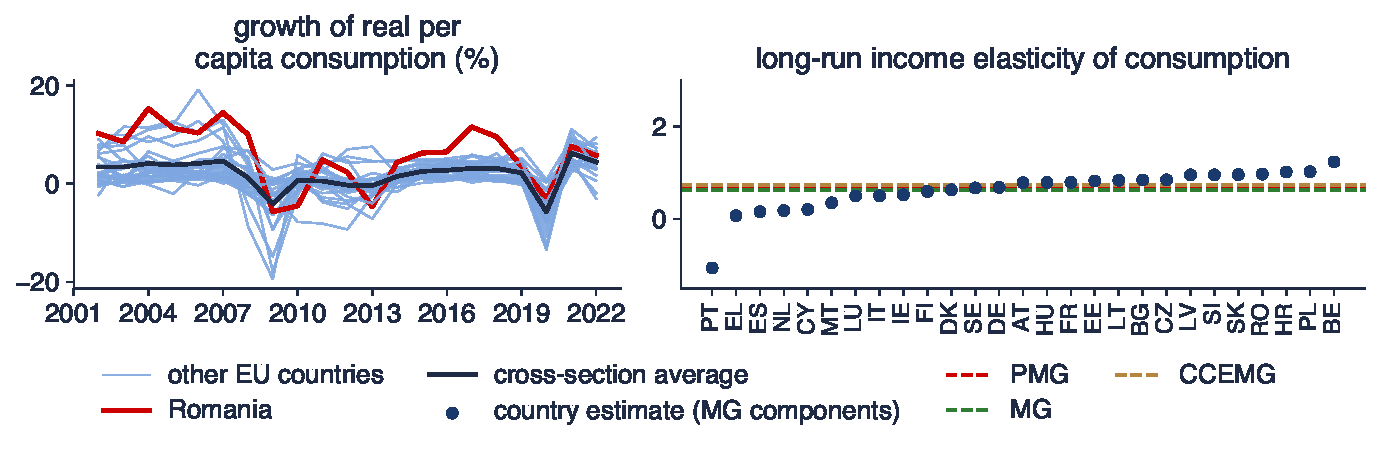
\includegraphics[width=0.97\textwidth,height=0.5\textheight,keepaspectratio]{ats_ch4_panel.pdf}
\end{center}
\vspace{-0.25cm}
\begin{itemize}
    \item Left: consumption growth (Romania in red, cross-section average in dark blue); right: country long-run income elasticities from the individual ARDLs, with MG, PMG and CCEMG
    \item Country elasticities range from \ensuremath{-}1.06 to 1.23; Romania 0.97
\end{itemize}
\quantlet{ATS\_ch4\_panel}{\qlurl{ATS_ch4_panel}}
\end{frame}

\begin{frame}{Long-run estimates for EU-27}
\itemsize{\small}
\begin{center}
\footnotesize
\begin{tabular}{lccc}
\toprule
\textbf{Estimator} & $\theta_y$ & $\theta_\pi$ & $\phi$ \\
\midrule
MG & 0.63 (0.09) & 0.82 (0.32) & \ensuremath{-}0.43 (0.032) \\
PMG & 0.69 (0.04) & 0.41 (0.18) & \ensuremath{-}0.31 (0.028) \\
dynamic FE & 0.81 (0.03) & 0.01 (0.23) & \ensuremath{-}0.29 (0.025) \\
group-mean DOLS & 0.77 (0.05) & \ensuremath{-}0.24 (0.17) & -- \\
CCEMG & 0.73 (0.05) & 0.10 (0.10) & -- \\
\bottomrule
\end{tabular}
\end{center}
\begin{itemize}
    \item Standard errors in brackets (MG, DOLS, CCEMG: dispersion of country estimates; PMG: likelihood; FE: clustered by country)
    \item Hausman MG against PMG: $H = 2.41$, $\chi^2(2)$, $p = 0.300$; CD of the PMG residuals: 30.9
\end{itemize}
\end{frame}

\begin{frame}{Interpreting the panel estimates}
\itemsize{\small}
\begin{itemize}
    \item The income elasticity lies between 0.63 (MG) and 0.81 (FE), clearly below one: consumption does not track income one for one over 2001--2022
    \item The Hausman test does not reject pooling, so PMG is the efficient choice for the income effect
    \item The inflation effect is not robust: its sign and size change with the estimator; do not report one of them alone
    \item PMG residuals remain strongly dependent (CD = 30.9): standard errors that ignore common shocks are too small; CCEMG is the safer benchmark
\end{itemize}
\end{frame}

\begin{frame}{Panel VAR in one slide}
\itemsize{\small}
\begin{itemize}
    \item $y_{it} = \mu_i + \sum_{j=1}^pA_jy_{i,t-j} + \varepsilon_{it}$: common dynamics, country fixed effects \refHNR
    \begin{itemize}
        \item $y_{it}$: the vector of variables of country $i$; $A_j$: lag matrices common to all countries; $\mu_i$: country fixed effects; $\varepsilon_{it}$: innovations
    \end{itemize}
    \item With small $T$ the within estimator is biased by $O(1/T)$ (Nickell); estimate by GMM on forward-orthogonal deviations with lagged levels as instruments \refAL
    \item Identification of shocks as in \atschlink{https://danpele.github.io/Advanced-Time-Series/EN/Courses/chapter3_structural_var_local_projections.pdf}{Chapter 3} (Cholesky, signs); impulse responses and FEVD are common to all countries
    \item Homogeneity of $A_j$ is the strong assumption: with macro panels of moderate $T$, mean-group VARs or CCE-augmented VARs are the heterogeneous alternatives
\end{itemize}
\end{frame}

\begin{frame}{Recap: Panel time series}
\itemsize{\small}
\begin{itemize}
    \item Test for cross-section dependence first; with strong dependence use CIPS and CCE, not LLC/IPS and pooled OLS
    \item Panel cointegration tests differ in their null and in the common-factor restriction; disagreement is informative
    \item MG for heterogeneity, PMG when theory pools the long run, Hausman to decide, CCE against common factors
\end{itemize}
\end{frame}


%=============================================================================
\section{AI for scientific discovery}
%=============================================================================

\begin{frame}{An open question}
\itemsize{\small}
\begin{itemize}
    \item Is the long-run pass-through of money-market rates to bank lending rates complete in Romania, and did it change after the 2022 tightening?
    \begin{itemize}
        \item formal: $H_0$: $\theta_{\text{lend}} = 1$ in a rank-2 VECM with ROBOR weakly exogenous; against a break in $\theta$ or in the markup in 2022
        \item falsified by a robust rejection: across pre-registered lag lengths, deterministic cases and bootstrap inference
    \end{itemize}
    \item Why it matters: the speed and completeness of pass-through decide how much the BNR must move its rate to move credit conditions
    \begin{itemize}
        \item literature to start from: \refdB, \refECR, \refJohD, \refCRT, \refPSSb
    \end{itemize}
\end{itemize}
\end{frame}

\begin{frame}{The discovery loop with an AI assistant}
\itemsize{\footnotesize}
\begin{itemize}
    \item An AI assistant (an LLM such as Claude, ChatGPT, Gemini or Copilot) speeds up each step; Semantic Scholar and Elicit help with the literature
    \begin{itemize}
        \item \textbf{literature}: \aiprompt{List peer-reviewed studies of interest-rate pass-through in Central and Eastern Europe that use cointegrated VARs or ARDL; give DOIs.} Then check every DOI on Crossref
        \item \textbf{hypothesis}: \aiprompt{Propose three reasons why lending-rate pass-through could exceed one, and one testable implication of each.}
        \item \textbf{code and replication}: ask for a Johansen function with restricted constant, then reproduce a known number first (the eigenvalues of this lecture)
        \item \textbf{robustness and critique}: \aiprompt{Act as a hostile referee: list every specification choice that could flip the complete pass-through test.}
    \end{itemize}
    \item Report: what was asked, what was kept, what was rejected (AI\_USE.md, AI\_ERRORS.md)
\end{itemize}
\end{frame}

\begin{frame}{What the human checks}
\itemsize{\small}
\begin{itemize}
    \item Every reference exists and says what is claimed (DOI resolves, title matches, the result is in the paper)
    \item The deterministic case of the critical values matches the estimated model (a frequent AI error: case-3 values for a case-2 model)
    \item The degrees of freedom of every LR test on $\beta$ and $\alpha$ are counted by hand
    \item Lag length, case, sample and the treatment of 2008--2009 are fixed before the results; all variants are reported
    \item A claim of ``complete pass-through'' is checked against the confidence set of $\theta$, not against one $p$-value
\end{itemize}
\end{frame}

\begin{frame}{Mini-case: the estimate is robust, the verdict is not}
\itemsize{\footnotesize}
\begin{center}
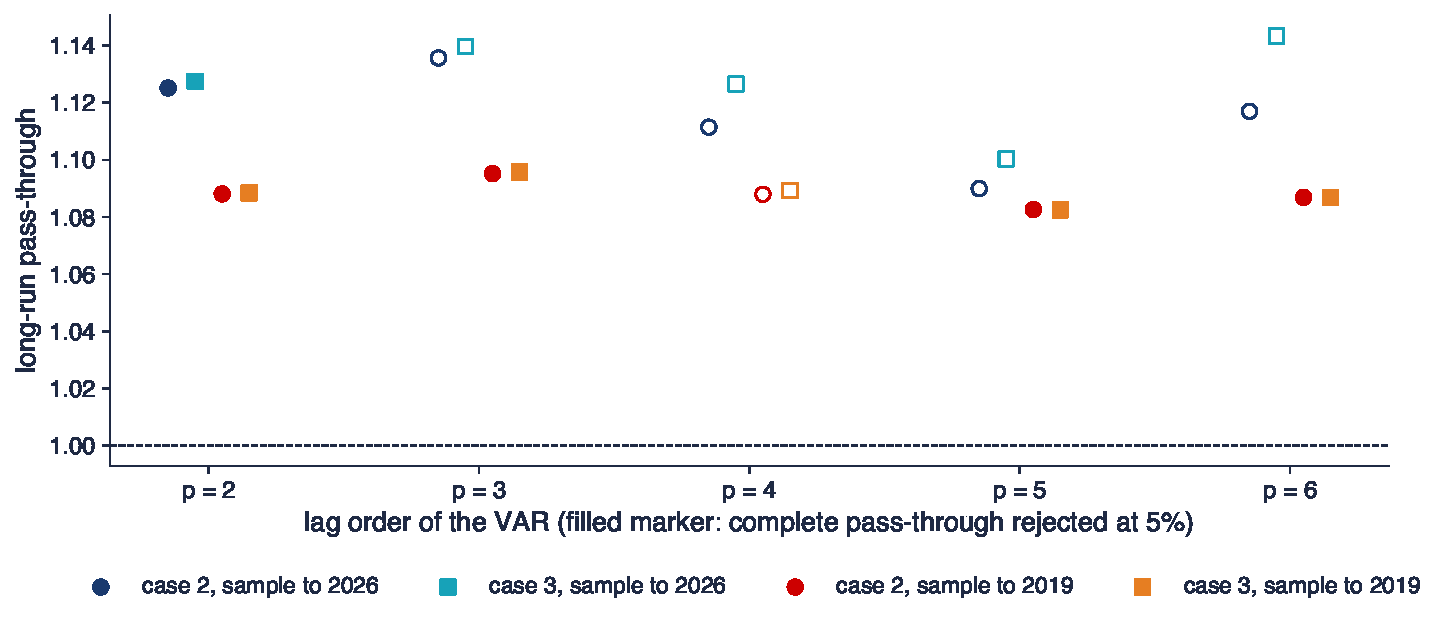
\includegraphics[width=0.97\textwidth,height=0.5\textheight,keepaspectratio]{ats_ch4_ai_case.pdf}
\end{center}
\vspace{-0.25cm}
\begin{itemize}
    \item Long-run pass-through to the lending rate in the rank-2 VECM: lags $p = 2, \dots, 6$, cases 2 and 3, samples ending in 2019 and in 2026; filled markers: $\theta = 1$ rejected at 5\%
    \item All 20 estimates lie between 1.08 and 1.14, yet complete pass-through is rejected in 10 of them: an AI summary that reports one $p$-value ``with confidence'' is wrong
\end{itemize}
\quantlet{ATS\_ch4\_ai\_robustness}{\qlurl{ATS_ch4_ai_robustness}}
\end{frame}

\begin{frame}{Project idea}
\itemsize{\small}
\begin{itemize}
    \item \textbf{Interest-rate pass-through in Central and Eastern Europe}: replicate first, then extend
    \begin{itemize}
        \item replicate: the Romanian rank-2 VECM of this lecture (eigenvalues 0.244, 0.177, 0.017) and the ARDL pass-through 1.15
        \item extend: Romania, Hungary, Czechia and Poland; broken constants \refJMN\ in 2008 and 2022; wild-bootstrap rank tests; PMG across countries with a Hausman test; NARDL for asymmetric pass-through
        \item pre-register: variables, sample, case, lag rule, rank procedure, the restrictions to test and the multiple-testing correction
    \end{itemize}
    \item Deliverables follow the course rules: repository, report, AI\_USE.md, AI\_ERRORS.md, oral defence
\end{itemize}
\end{frame}


%=============================================================================
\section{Wrap-up}
%=============================================================================

\begin{frame}{Key takeaways}
\itemsize{\small}
\begin{itemize}
    \item Johansen = reduced-rank regression; the rank test is non-standard, depends on the case and over-rejects in small samples
    \item Given the rank, restrictions on $\beta$ (economics) and $\alpha$ (weak exogeneity) are ordinary $\chi^2$ tests
    \item Cointegration supplies long-run zeros for structural analysis: permanent and transitory shocks
    \item ARDL is a conditional VECM: valid under weak exogeneity and a single relation, with small-sample bounds
    \item Panels add power but bring heterogeneity and cross-section dependence: CD first, then CIPS, MG/PMG and CCE
\end{itemize}
\end{frame}

\begin{frame}{Self-assessment}
\itemsize{\small}
\begin{columns}[T]
\begin{column}{0.56\textwidth}
\begin{block}{Questions}
\begin{itemize}
    \item Why does one eigen-decomposition give the ML estimator of $\beta$ for every rank?
    \item Which deterministic case fits two interest rates without drift?
    \item How many degrees of freedom has the test of a known $\beta$ with $n_1 = 3$, $r = 2$?
    \item What does weak exogeneity of ROBOR allow you to do?
    \item Why can IPS reject a unit root that CIPS does not reject?
\end{itemize}
\end{block}
\end{column}
\begin{column}{0.40\textwidth}
\begin{block}{Next: \atschlink{https://danpele.github.io/Advanced-Time-Series/EN/Courses/chapter5_bvar_factor_models_nowcasting.pdf}{Chapter 5}}
\begin{itemize}
    \item Bayesian VAR, factor models and nowcasting
    \item Shrinkage handles the parameter problem we met in small samples; factors generalise the cross-section averages of CCE
\end{itemize}
\end{block}
\end{column}
\end{columns}
\end{frame}


%=============================================================================
\section{Appendix}
%=============================================================================

\begin{frame}{Appendix: from the likelihood to the eigenvalues}
\hypertarget{atsapp1}{}\atsappback{atssrc1}{Back}
\itemsize{\small}
\begin{itemize}
    \item For fixed $\beta$: $|\hat\Omega(\beta)| = |S_{00} - S_{01}\beta(\beta'S_{11}\beta)^{-1}\beta'S_{10}|$; apply the partitioned determinant to $\begin{pmatrix}S_{00} & S_{01}\beta\\ \beta'S_{10} & \beta'S_{11}\beta\end{pmatrix}$ in both orders
    \item $|\hat\Omega(\beta)|\,|\beta'S_{11}\beta| = |S_{00}|\,|\beta'(S_{11} - S_{10}S_{00}^{-1}S_{01})\beta|$, which gives the ratio on the slide
    \item Write $\beta = S_{11}^{-1/2}\eta$: the ratio becomes $|\eta'(I - M)\eta|/|\eta'\eta|$ with $M = S_{11}^{-1/2}S_{10}S_{00}^{-1}S_{01}S_{11}^{-1/2}$; it is minimised by the eigenvectors of $M$ with the $r$ largest eigenvalues
    \item The minimum is $\prod_{i\le r}(1 - \lambda_i)$; nested ranks share eigenvectors, so the LR statistics are sums of $-T\ln(1 - \hat\lambda_i)$
\end{itemize}
\end{frame}

\begin{frame}{Appendix: why $C = \beta_\perp(\alpha_\perp'\Gamma\beta_\perp)^{-1}\alpha_\perp'$}
\hypertarget{atsapp2}{}\atsappback{atssrc1}{Back}
\itemsize{\small}
\begin{itemize}
    \item Multiply the VECM by $\alpha_\perp'$: $\alpha_\perp'\Delta y_t = \alpha_\perp'\sum_i\Gamma_i\Delta y_{t-i} + \alpha_\perp'\varepsilon_t$; summing gives $\alpha_\perp'\Gamma y_t \approx \alpha_\perp'\sum_{s\le t}\varepsilon_s$ up to stationary terms
    \item Decompose $y_t = \beta(\beta'\beta)^{-1}\beta'y_t + \beta_\perp(\beta_\perp'\beta_\perp)^{-1}\beta_\perp'y_t$; the first part is stationary
    \item Hence $\alpha_\perp'\Gamma\beta_\perp\,(\beta_\perp'\beta_\perp)^{-1}\beta_\perp'y_t \approx \alpha_\perp'\sum_s\varepsilon_s$; invert $\alpha_\perp'\Gamma\beta_\perp$ (the I(1) condition) and premultiply by $\beta_\perp$
    \item Result: the non-stationary part of $y_t$ is $\beta_\perp(\alpha_\perp'\Gamma\beta_\perp)^{-1}\alpha_\perp'\sum_s\varepsilon_s = C\sum_s\varepsilon_s$
\end{itemize}
\end{frame}

\begin{frame}{Appendix: the PMG likelihood}
\hypertarget{atsapp3}{}\atsappback{atssrc1}{Back}
\itemsize{\small}
\begin{itemize}
    \item $\ell(\theta, \phi, \sigma^2) = -\sum_{i=1}^N\frac{T_i}{2}\ln(2\pi\sigma_i^2) - \sum_{i=1}^N\frac{1}{2\sigma_i^2}(\Delta y_i - \phi_i\xi_i(\theta))'H_i(\Delta y_i - \phi_i\xi_i(\theta))$
    \item $\xi_i(\theta) = y_{i,-1} - X_{i,-1}\theta$; $H_i$ projects out the country's short-run regressors and intercept
    \item Given $\theta$, $\phi_i$ and $\sigma_i^2$ are country OLS; the concentrated likelihood $-\sum_i\frac{T_i}{2}\ln\hat\sigma_i^2(\theta)$ is maximised over $\theta$ (back-substitution or Newton)
    \item $\hat\theta_{PMG}$ is consistent and asymptotically normal if $\phi_i < 0$ for all $i$ and the long run is homogeneous; the I(0)/I(1) status of $x$ does not matter, as in ARDL
\end{itemize}
\end{frame}


%=============================================================================
\section{References}
%=============================================================================

\begin{frame}{References (1/5)}
\itemsize{\tiny}
\begin{itemize}
    \item Abrigo, M. R. M., \& Love, I. (2016). Estimation of panel vector autoregression in Stata. \textit{The Stata Journal}, 16(3), 778--804. \href{https://doi.org/10.1177/1536867X1601600314}{doi:10.1177/1536867X1601600314}
    \item Bacon, R. W. (1991). Rockets and feathers: The asymmetric speed of adjustment of UK retail gasoline prices to cost changes. \textit{Energy Economics}, 13(3), 211--218. \href{https://doi.org/10.1016/0140-9883(91)90022-R}{doi:10.1016/0140-9883(91)90022-R}
    \item Breitung, J., \& Pesaran, M. H. (2008). Unit roots and cointegration in panels. In L. Mátyás \& P. Sevestre (Eds.), \textit{The Econometrics of Panel Data} (pp.\ 279--322). Springer. \href{https://doi.org/10.1007/978-3-540-75892-1_9}{doi:10.1007/978-3-540-75892-1\_9}
    \item Cavaliere, G., Rahbek, A., \& Taylor, A. M. R. (2010). Cointegration rank testing under conditional heteroskedasticity. \textit{Econometric Theory}, 26(6), 1719--1760. \href{https://doi.org/10.1017/S0266466609990776}{doi:10.1017/S0266466609990776}
    \item Cavaliere, G., Rahbek, A., \& Taylor, A. M. R. (2012). Bootstrap determination of the co-integration rank in vector autoregressive models. \textit{Econometrica}, 80(4), 1721--1740. \href{https://doi.org/10.3982/ECTA9099}{doi:10.3982/ECTA9099}
    \item Chudik, A., \& Pesaran, M. H. (2015). Common correlated effects estimation of heterogeneous dynamic panel data models with weakly exogenous regressors. \textit{Journal of Econometrics}, 188(2), 393--420. \href{https://doi.org/10.1016/j.jeconom.2015.03.007}{doi:10.1016/j.jeconom.2015.03.007}
    \item de Bondt, G. J. (2005). Interest rate pass-through: Empirical results for the euro area. \textit{German Economic Review}, 6(1), 37--78. \href{https://doi.org/10.1111/j.1465-6485.2005.00121.x}{doi:10.1111/j.1465-6485.2005.00121.x}
    \item Égert, B., Crespo-Cuaresma, J., \& Reininger, T. (2007). Interest rate pass-through in Central and Eastern Europe: Reborn from ashes merely to pass away? \textit{Journal of Policy Modeling}, 29(2), 209--225. \href{https://doi.org/10.1016/j.jpolmod.2007.01.005}{doi:10.1016/j.jpolmod.2007.01.005}
    \item Engle, R. F., \& Granger, C. W. J. (1987). Co-integration and error correction: Representation, estimation, and testing. \textit{Econometrica}, 55(2), 251--276. \href{https://doi.org/10.2307/1913236}{doi:10.2307/1913236}
    \item Gonzalo, J., \& Ng, S. (2001). A systematic framework for analyzing the dynamic effects of permanent and transitory shocks. \textit{Journal of Economic Dynamics and Control}, 25(10), 1527--1546. \href{https://doi.org/10.1016/S0165-1889(99)00062-7}{doi:10.1016/S0165-1889(99)00062-7}
    \item Hamilton, J. D. (1994). \textit{Time Series Analysis}. Princeton University Press. \href{https://doi.org/10.2307/j.ctv14jx6sm}{doi:10.2307/j.ctv14jx6sm}
    \item Holtz-Eakin, D., Newey, W., \& Rosen, H. S. (1988). Estimating vector autoregressions with panel data. \textit{Econometrica}, 56(6), 1371--1395. \href{https://doi.org/10.2307/1913103}{doi:10.2307/1913103}
\end{itemize}
\end{frame}

\begin{frame}{References (2/5)}
\itemsize{\tiny}
\begin{itemize}
    \item Im, K. S., Pesaran, M. H., \& Shin, Y. (2003). Testing for unit roots in heterogeneous panels. \textit{Journal of Econometrics}, 115(1), 53--74. \href{https://doi.org/10.1016/S0304-4076(03)00092-7}{doi:10.1016/S0304-4076(03)00092-7}
    \item Johansen, S. (1988). Statistical analysis of cointegration vectors. \textit{Journal of Economic Dynamics and Control}, 12(2--3), 231--254. \href{https://doi.org/10.1016/0165-1889(88)90041-3}{doi:10.1016/0165-1889(88)90041-3}
    \item Johansen, S. (1991). Estimation and hypothesis testing of cointegration vectors in Gaussian vector autoregressive models. \textit{Econometrica}, 59(6), 1551--1580. \href{https://doi.org/10.2307/2938278}{doi:10.2307/2938278}
    \item Johansen, S. (1992). Determination of cointegration rank in the presence of a linear trend. \textit{Oxford Bulletin of Economics and Statistics}, 54(3), 383--397. \href{https://doi.org/10.1111/j.1468-0084.1992.tb00008.x}{doi:10.1111/j.1468-0084.1992.tb00008.x}
    \item Johansen, S. (1995a). \textit{Likelihood-Based Inference in Cointegrated Vector Autoregressive Models}. Oxford University Press. \href{https://doi.org/10.1093/0198774508.001.0001}{doi:10.1093/0198774508.001.0001}
    \item Johansen, S. (1995b). Identifying restrictions of linear equations with applications to simultaneous equations and cointegration. \textit{Journal of Econometrics}, 69(1), 111--132. \href{https://doi.org/10.1016/0304-4076(94)01664-L}{doi:10.1016/0304-4076(94)01664-L}
    \item Johansen, S. (1995c). A statistical analysis of cointegration for I(2) variables. \textit{Econometric Theory}, 11(1), 25--59. \href{https://doi.org/10.1017/S0266466600009026}{doi:10.1017/S0266466600009026}
    \item Johansen, S. (2002). A small sample correction for the test of cointegrating rank in the vector autoregressive model. \textit{Econometrica}, 70(5), 1929--1961. \href{https://doi.org/10.1111/1468-0262.00358}{doi:10.1111/1468-0262.00358}
    \item Johansen, S., \& Juselius, K. (1990). Maximum likelihood estimation and inference on cointegration, with applications to the demand for money. \textit{Oxford Bulletin of Economics and Statistics}, 52(2), 169--210. \href{https://doi.org/10.1111/j.1468-0084.1990.mp52002003.x}{doi:10.1111/j.1468-0084.1990.mp52002003.x}
    \item Johansen, S., Mosconi, R., \& Nielsen, B. (2000). Cointegration analysis in the presence of structural breaks in the deterministic trend. \textit{The Econometrics Journal}, 3(2), 216--249. \href{https://doi.org/10.1111/1368-423X.00047}{doi:10.1111/1368-423X.00047}
    \item Juselius, K. (2006). \textit{The Cointegrated VAR Model: Methodology and Applications}. Oxford University Press. \href{https://doi.org/10.1093/oso/9780199285662.001.0001}{doi:10.1093/oso/9780199285662.001.0001}
    \item Kao, C. (1999). Spurious regression and residual-based tests for cointegration in panel data. \textit{Journal of Econometrics}, 90(1), 1--44. \href{https://doi.org/10.1016/S0304-4076(98)00023-2}{doi:10.1016/S0304-4076(98)00023-2}
\end{itemize}
\end{frame}

\begin{frame}{References (3/5)}
\itemsize{\tiny}
\begin{itemize}
    \item Kapetanios, G., Pesaran, M. H., \& Yamagata, T. (2011). Panels with non-stationary multifactor error structures. \textit{Journal of Econometrics}, 160(2), 326--348. \href{https://doi.org/10.1016/j.jeconom.2010.10.001}{doi:10.1016/j.jeconom.2010.10.001}
    \item Kilian, L., \& Lütkepohl, H. (2017). \textit{Structural Vector Autoregressive Analysis}. Cambridge University Press. \href{https://doi.org/10.1017/9781108164818}{doi:10.1017/9781108164818}
    \item King, R. G., Plosser, C. I., Stock, J. H., \& Watson, M. W. (1991). Stochastic trends and economic fluctuations. \textit{American Economic Review}, 81(4), 819--840. \href{https://www.jstor.org/stable/2006644}{jstor.org}
    \item Kripfganz, S., \& Schneider, D. C. (2020). Response surface regressions for critical value bounds and approximate p-values in equilibrium correction models. \textit{Oxford Bulletin of Economics and Statistics}, 82(6), 1456--1481. \href{https://doi.org/10.1111/obes.12377}{doi:10.1111/obes.12377}
    \item Levin, A., Lin, C.-F., \& Chu, C.-S. J. (2002). Unit root tests in panel data: Asymptotic and finite-sample properties. \textit{Journal of Econometrics}, 108(1), 1--24. \href{https://doi.org/10.1016/S0304-4076(01)00098-7}{doi:10.1016/S0304-4076(01)00098-7}
    \item Lütkepohl, H. (2005). \textit{New Introduction to Multiple Time Series Analysis}. Springer. \href{https://doi.org/10.1007/978-3-540-27752-1}{doi:10.1007/978-3-540-27752-1}
    \item MacKinnon, J. G., Haug, A. A., \& Michelis, L. (1999). Numerical distribution functions of likelihood ratio tests for cointegration. \textit{Journal of Applied Econometrics}, 14(5), 563--577. \href{https://doi.org/10.1002/(SICI)1099-1255(199909/10)14:5\%3C563::AID-JAE530\%3E3.0.CO\%3B2-R}{doi:10.1002/(SICI)1099-1255(199909/10)14:5\textless{}563::AID-JAE530\textgreater{}3.0.CO;2-R}
    \item Narayan, P. K. (2005). The saving and investment nexus for China: Evidence from cointegration tests. \textit{Applied Economics}, 37(17), 1979--1990. \href{https://doi.org/10.1080/00036840500278103}{doi:10.1080/00036840500278103}
    \item Nickell, S. (1981). Biases in dynamic models with fixed effects. \textit{Econometrica}, 49(6), 1417--1426. \href{https://doi.org/10.2307/1911408}{doi:10.2307/1911408}
    \item Osterwald-Lenum, M. (1992). A note with quantiles of the asymptotic distribution of the maximum likelihood cointegration rank test statistics. \textit{Oxford Bulletin of Economics and Statistics}, 54(3), 461--472. \href{https://doi.org/10.1111/j.1468-0084.1992.tb00013.x}{doi:10.1111/j.1468-0084.1992.tb00013.x}
    \item Pantula, S. G. (1989). Testing for unit roots in time series data. \textit{Econometric Theory}, 5(2), 256--271. \href{https://doi.org/10.1017/S0266466600012421}{doi:10.1017/S0266466600012421}
    \item Pedroni, P. (1999). Critical values for cointegration tests in heterogeneous panels with multiple regressors. \textit{Oxford Bulletin of Economics and Statistics}, 61(S1), 653--670. \href{https://doi.org/10.1111/1468-0084.0610s1653}{doi:10.1111/1468-0084.0610s1653}
\end{itemize}
\end{frame}

\begin{frame}{References (4/5)}
\itemsize{\tiny}
\begin{itemize}
    \item Pedroni, P. (2001). Purchasing power parity tests in cointegrated panels. \textit{The Review of Economics and Statistics}, 83(4), 727--731. \href{https://doi.org/10.1162/003465301753237803}{doi:10.1162/003465301753237803}
    \item Pedroni, P. (2004). Panel cointegration: Asymptotic and finite sample properties of pooled time series tests with an application to the PPP hypothesis. \textit{Econometric Theory}, 20(3), 597--625. \href{https://doi.org/10.1017/S0266466604203073}{doi:10.1017/S0266466604203073}
    \item Pesaran, M. H. (2006). Estimation and inference in large heterogeneous panels with a multifactor error structure. \textit{Econometrica}, 74(4), 967--1012. \href{https://doi.org/10.1111/j.1468-0262.2006.00692.x}{doi:10.1111/j.1468-0262.2006.00692.x}
    \item Pesaran, M. H. (2007). A simple panel unit root test in the presence of cross-section dependence. \textit{Journal of Applied Econometrics}, 22(2), 265--312. \href{https://doi.org/10.1002/jae.951}{doi:10.1002/jae.951}
    \item Pesaran, M. H. (2015a). Testing weak cross-sectional dependence in large panels. \textit{Econometric Reviews}, 34(6--10), 1089--1117. \href{https://doi.org/10.1080/07474938.2014.956623}{doi:10.1080/07474938.2014.956623}
    \item Pesaran, M. H. (2015b). \textit{Time Series and Panel Data Econometrics}. Oxford University Press. \href{https://doi.org/10.1093/acprof:oso/9780198736912.001.0001}{doi:10.1093/acprof:oso/9780198736912.001.0001}
    \item Pesaran, M. H. (2021). General diagnostic tests for cross-sectional dependence in panels. \textit{Empirical Economics}, 60(1), 13--50. \href{https://doi.org/10.1007/s00181-020-01875-7}{doi:10.1007/s00181-020-01875-7}
    \item Pesaran, M. H., \& Shin, Y. (1998). An autoregressive distributed-lag modelling approach to cointegration analysis. In S. Strøm (Ed.), \textit{Econometrics and Economic Theory in the 20th Century: The Ragnar Frisch Centennial Symposium} (pp.\ 371--413). Cambridge University Press. \href{https://doi.org/10.1017/CCOL0521633230.011}{doi:10.1017/CCOL0521633230.011}
    \item Pesaran, M. H., Shin, Y., \& Smith, R. J. (2001). Bounds testing approaches to the analysis of level relationships. \textit{Journal of Applied Econometrics}, 16(3), 289--326. \href{https://doi.org/10.1002/jae.616}{doi:10.1002/jae.616}
    \item Pesaran, M. H., Shin, Y., \& Smith, R. P. (1999). Pooled mean group estimation of dynamic heterogeneous panels. \textit{Journal of the American Statistical Association}, 94(446), 621--634. \href{https://doi.org/10.1080/01621459.1999.10474156}{doi:10.1080/01621459.1999.10474156}
    \item Pesaran, M. H., \& Smith, R. (1995). Estimating long-run relationships from dynamic heterogeneous panels. \textit{Journal of Econometrics}, 68(1), 79--113. \href{https://doi.org/10.1016/0304-4076(94)01644-F}{doi:10.1016/0304-4076(94)01644-F}
    \item Phillips, P. C. B., \& Hansen, B. E. (1990). Statistical inference in instrumental variables regression with I(1) processes. \textit{The Review of Economic Studies}, 57(1), 99--125. \href{https://doi.org/10.2307/2297545}{doi:10.2307/2297545}
\end{itemize}
\end{frame}

\begin{frame}{References (5/5)}
\itemsize{\tiny}
\begin{itemize}
    \item Phillips, P. C. B., \& Moon, H. R. (1999). Linear regression limit theory for nonstationary panel data. \textit{Econometrica}, 67(5), 1057--1111. \href{https://doi.org/10.1111/1468-0262.00070}{doi:10.1111/1468-0262.00070}
    \item Reinsel, G. C., \& Ahn, S. K. (1992). Vector autoregressive models with unit roots and reduced rank structure: Estimation, likelihood ratio test, and forecasting. \textit{Journal of Time Series Analysis}, 13(4), 353--375. \href{https://doi.org/10.1111/j.1467-9892.1992.tb00113.x}{doi:10.1111/j.1467-9892.1992.tb00113.x}
    \item Saikkonen, P. (1991). Asymptotically efficient estimation of cointegration regressions. \textit{Econometric Theory}, 7(1), 1--21. \href{https://doi.org/10.1017/S0266466600004217}{doi:10.1017/S0266466600004217}
    \item Shin, Y., Yu, B., \& Greenwood-Nimmo, M. (2014). Modelling asymmetric cointegration and dynamic multipliers in a nonlinear ARDL framework. In R. C. Sickles \& W. C. Horrace (Eds.), \textit{Festschrift in Honor of Peter Schmidt} (pp.\ 281--314). Springer. \href{https://doi.org/10.1007/978-1-4899-8008-3_9}{doi:10.1007/978-1-4899-8008-3\_9}
    \item Stock, J. H., \& Watson, M. W. (1993). A simple estimator of cointegrating vectors in higher order integrated systems. \textit{Econometrica}, 61(4), 783--820. \href{https://doi.org/10.2307/2951763}{doi:10.2307/2951763}
    \item Swensen, A. R. (2006). Bootstrap algorithms for testing and determining the cointegration rank in VAR models. \textit{Econometrica}, 74(6), 1699--1714. \href{https://doi.org/10.1111/j.1468-0262.2006.00723.x}{doi:10.1111/j.1468-0262.2006.00723.x}
    \item Toda, H. Y., \& Yamamoto, T. (1995). Statistical inference in vector autoregressions with possibly integrated processes. \textit{Journal of Econometrics}, 66(1--2), 225--250. \href{https://doi.org/10.1016/0304-4076(94)01616-8}{doi:10.1016/0304-4076(94)01616-8}
    \item Westerlund, J. (2007). Testing for error correction in panel data. \textit{Oxford Bulletin of Economics and Statistics}, 69(6), 709--748. \href{https://doi.org/10.1111/j.1468-0084.2007.00477.x}{doi:10.1111/j.1468-0084.2007.00477.x}
\end{itemize}
\end{frame}

\end{document}
